% Compatibility for the publisher's legacy rQUF2e class on modern LaTeX.
% Save kernel lifecycle/output commands; retain publisher fonts and layout.
\makeatletter
\let\QFKernelDocument\document
\let\QFKernelEndDocument\enddocument
\let\QFKernelOutputPage\@outputpage
\makeatother
\documentclass{rQUF2e}
\makeatletter
\let\document\QFKernelDocument
\let\enddocument\QFKernelEndDocument
\let\@outputpage\QFKernelOutputPage
\makeatother

\usepackage{booktabs,threeparttable,longtable,array,tabularx,multirow}
\usepackage{xcolor}
\usepackage{url}
\newcommand{\href}[2]{#2}
\providecommand{\theHtable}{}
\emergencystretch=2em
\newtheorem{proposition}{Proposition}
\newtheorem{corollary}{Corollary}
\newcommand{\E}{\mathbb{E}}
\newcommand{\Pp}{\mathbb{P}}
\newcommand{\Loss}{\mathcal{L}}
\newcommand{\Kset}{\mathcal{K}}
\newenvironment{widefigure}[1][!tbp]{\begin{figure}[#1]}{\end{figure}}
\newenvironment{widetable}[1][!tbp]{\begin{table}[#1]}{\end{table}}
\setcounter{topnumber}{3}\setcounter{bottomnumber}{2}\setcounter{totalnumber}{4}
\renewcommand{\topfraction}{0.9}\renewcommand{\bottomfraction}{0.8}
\renewcommand{\textfraction}{0.08}\renewcommand{\floatpagefraction}{0.85}
\bibpunct{(}{)}{,}{a}{}{,}
% The official legacy class defaults to a fictional 'To appear' header and received dates.
% Keep its layout and source unmodified; use ordinary manuscript pagination instead.
\makeatletter
\def\ps@qfmanuscript{\let\@oddhead\@empty\let\@evenhead\@empty
 \def\@oddfoot{\hfil\thepage\hfil}\let\@evenfoot\@oddfoot}
\let\ps@plain\ps@qfmanuscript
\makeatother
\pagestyle{qfmanuscript}
\makeatletter\def\trimmarks{}\makeatother
% Restore space for manuscript page numbers after replacing the legacy output routine.
\addtolength{\textheight}{-16pt}
\setlength{\footskip}{20pt}
\begin{document}
\title{Latent Dimension Selection in Neural Asset Pricing: Sensitivity and Pricing-Loss Costs}
\author{JINPENG WANG$\dag$ and YAN JIANG$^{\ast}\dag$\thanks{$^\ast$Corresponding author. Email: jiangyan@gcu.edu.cn. Author ORCIDs: Jinpeng Wang, 0009-0003-7324-2211; Yan Jiang, 0009-0004-0250-7486.}}
\affil{$\dag$International Business School, Guangzhou City University of Technology,\\
No. 1 Xuefu Road, Guangzhou 510800, China}
\received{Author manuscript; not accepted for publication}

\maketitle
\begin{abstract}
A selected latent dimension summarizes a model under an evaluation task, but does not alone identify priced risks. We audit this distinction using archived U.S. equity pricing networks, matched controls, conditional autoencoders, and known-truth simulations. For combined Core-86 assets, transferring the HJ-preferred four factors to equal-moment evaluation increases the pricing norm by 19.7\%, whereas transferring the equal-moment-preferred two factors to HJ increases it by 1.9\%. A same-panel six-feature ablation does not reproduce the archived pipeline reversal. An audit reproduces all 900 archived conditional-autoencoder and linear-loading surface rows. The autoencoder prefers eight factors, the grid upper bound, across all 15 asset--weight tasks; its five-factor excess ranges from 2.35\% to 11.17\%. Linear loadings select four, five or eight factors, with endpoint-transfer costs from 2.09\% to 9.34\%. Thus objective sensitivity is not universal across the tested architectures. These retrospective norm costs are neither investor return losses nor validated significance findings. Simulations demonstrate possible selection mechanisms, while market-direction evidence remains imprecise. We distinguish candidate selection, representation concentration and economic risk counts.
\end{abstract}
\begin{keywords}
Machine learning; Asset pricing; Pricing dimension; Model comparison; Representation geometry; Feature ablation
\end{keywords}
\begin{classcode}G12; C52; C53; C55\end{classcode}
\raggedbottom
\section{Introduction}
Choosing a latent dimension is an operational step in neural asset pricing: the researcher must decide how many factors to retain and which pricing errors matter for that choice. The practical question is whether a dimension selected under one evaluation task remains useful under another, and how much pricing fit is sacrificed when it does not. A change in the identity of the minimum is insufficient: a near tie and a large deterioration have different implications.

We distinguish three quantities: concentration in hidden activations, the factor count minimizing a specified empirical pricing loss, and the number of structural priced risks. Flexible predictors and characteristic-based factor models address related but different tasks \citep{kelly2019characteristics,gu2020empirical,gu2021autoencoder,chen2024deep}. We do not claim that these studies mistake prediction for structural identification. Our contribution is a bounded empirical audit of how the first two quantities behave under explicitly stated comparisons.

The original diagnostic networks provide complete candidate loss profiles across three asset spans, six dimensions, five initializations and 21 evaluation weights. We use those frozen profiles to report both preferred dimensions and the cost of carrying the preferred dimension from one endpoint to the other. Cost means additional pricing norm on the same evaluation sample, not a welfare loss or prospective investment outcome. The comparisons are retrospective; the sample minimum is not an oracle population benchmark.

The evidence separates controlled variation from bundled variation. Changing evaluation weights within a fixed model family isolates the sensitivity of the evaluation criterion. The archived characteristic-pipeline comparison also changes construction, coverage and timing, so it cannot identify a feature-deletion effect. A later same-panel deletion control does not reproduce that pipeline reversal. Market hedging and spectral diagnostics provide clues about payoff directions, but wide intervals prevent a precise economic attribution.

A conditional-autoencoder extension tests a boundary of the original narrative. Eight factors, the upper candidate-grid endpoint, win 87.2\% of development resampling draws. The complete archived secondary grid also selects eight in all fifteen autoencoder asset--weight tasks, while the matched linear-loading winners vary. The five-factor candidate has a development pricing norm 11.2\% above the eight-factor candidate; the corresponding excess for linear loadings is only 1.4\%. These are conditional descriptive differences, not significant performance or equivalence findings. A known-truth calibration shows that the new simultaneous intervals undercover, and we do not use them to establish equivalence or structural nonidentification.

Related work in this journal provides useful distinctions. \citet{lo2023qf} study risk-premium prediction and local prediction explanations, whereas our object is the interpretation and cost of candidate factor counts. \citet{xu2024qf} show the importance of a demanding benchmark when assessing machine-learning forecasts. \citet{jiang2025qf} develop a factor-model test; we do not propose a replacement test. \citet{dom2025qf} show that covariance-estimator comparisons depend on portfolio construction. Our related concern is the dependence of latent-dimension comparisons on evaluation design, without claiming that a change of objective producing a different optimum is itself a new theorem.

The study is limited to the archived model families and historical data. The original networks failed earlier benchmark-advancement criteria; the conditional-autoencoder control is exploratory and does not access 2020--2025. Simulations demonstrate possible mechanisms, not their empirical causal prevalence. The following sections define the objects, describe the data and chronology, report candidate losses and controls, and assess the narrower role of representation geometry. The separate updating replay remains in the previously archived supplement and is outside the main research question.

\section{Related literature and conceptual framework}

\subsection{Flexible prediction and structural pricing objects}

Machine-learning asset pricing has developed along two related lines. The first uses firm characteristics and flexible interactions to predict individual-stock returns \citep{gu2020empirical,leippold2022machine,avramov2023machine}. The second uses characteristics to estimate time-varying exposures, latent factors, or stochastic discount factors (SDFs) \citep{kelly2019characteristics,gu2021autoencoder,chen2024deep,feng2024deep}. Surveys emphasize that these methods can improve prediction and pricing while accommodating a much larger information set than conventional linear specifications \citep{karolyi2020new,giglio2022factor,bagnara2024review}. Recent work also develops formal significance and model-selection procedures for neural or high-dimensional pricing models \citep{fallahgoul2024significance,feng2026stepwise}.

These results establish the value of flexible functional forms, but they do not make the size of a hidden layer or a fitted bottleneck an economic primitive. A predictor can reduce conditional mean-squared error without spanning an SDF that prices a given asset set. A network with many parameters can generate a concentrated representation, while a compact representation can omit a weakly priced direction. We therefore separate predictive complexity, representation dimension, factor dimension, and pricing dimension, and evaluate each with an object-specific criterion.

Let $Z_t\in\mathbb{R}^{N_t\times p}$ denote the characteristic panel at date $t$, $h_{K,s}(Z_t)$ a fitted representation with nominal output dimension $K$ and training seed $s$, and $F_{K,s,t+1}$ the resulting factor return or SDF innovation. For test-asset excess returns $R_{t+1}\in\mathbb{R}^{J}$, define pricing moments
\begin{equation}
 g_{K,s}=\E[m_{K,s,t+1}R_{t+1}],
\end{equation}
where $m_{K,s,t+1}$ is the scaled SDF associated with the fitted factors. For a positive semidefinite weighting matrix $W$, the population pricing loss is
\begin{equation}
 \Loss_W(K,s)=g_{K,s}'Wg_{K,s}.
 \label{eq:pricing-loss}
\end{equation}
The empirically preferred candidate dimension is an argmin of an estimate of Eq.~\eqref{eq:pricing-loss}; it need not be a pricing-sufficient or structurally minimal dimension. It is indexed by $W$, the asset vector $R$, the information set used to construct $h$, the fitting sample, and algorithmic randomness. Without additional restrictions it is not an invariant property of the economy.

\subsection{Latent-factor dimension and weak priced directions}

The econometric literature offers consistent procedures for counting pervasive factors from the eigenvalues of large panels \citep{bai2002factors,onatski2010factors,ahn2013eigenvalue}. Asset-pricing applications, however, attach an additional requirement: a direction must matter for pricing, not merely explain covariance. Characteristic-based factor models and supervised latent-factor methods make this distinction operational \citep{kelly2019characteristics,lettau2020factors}. It becomes especially important when risk prices are weak, when the candidate family is nested, or when additional factors are nearly redundant.

Our question is therefore different from estimating the statistical rank of returns. We ask whether the \emph{smallest pricing-sufficient dimension} can be recovered from feasible out-of-sample losses. Cross-validation is well suited to prediction, but selection of a uniquely minimal model requires stronger separation conditions \citep{shao1993cv,yang2007cv,arlot2010cv}. Proposition~\ref{prop:inconsistency} specializes this point to nested pricing models: when larger models share the same population pricing loss and differ only at a higher stochastic order, the raw validation minimum can continue to overselect with positive probability. The simulation section evaluates the size of that problem under controlled truth.

\subsection{Test assets, weighting geometry, and what is identified}

Classical asset-pricing tests make clear that an SDF is assessed through moment restrictions and that the economic distance from a model depends on the return space and its weighting \citep{gibbons1989test,hansen1991implications,shanken1992beta,hansen1997assessing}. Two-pass inference and specification tests further depend on estimated betas, risk prices, and their sampling error \citep{fama1992cross,jagannathan1996conditional,kan2013pricing}. The choice of test assets is consequential: apparently strong fit can arise when the portfolios have a low-dimensional covariance structure or weak exposure to the disputed direction \citep{lewellen2010skeptical}.

These observations imply that a pricing dimension cannot be reported without its measurement geometry. An equal-weighted loss assigns the same coordinate weight to each sample moment. An HJ-type loss rotates and rescales the moment vector using a return second-moment matrix. The factor sets of \citet{fama1993common} and \citet{fama2015five}, characteristic-sorted portfolios, and individual stocks expose different directions. We therefore cross test dimension choices across asset systems and weighting matrices. Disagreement describes the task dependence of the fitted comparison. By itself it neither identifies a structural dimension nor shows that an invariant economic object does not exist.

\subsection{Factor proliferation, model search, and reproducibility}

The factor-zoo literature shows that searching a large menu requires multiple-testing control, shrinkage, and external replication \citep{harvey2016cross,feng2020taming,hou2020replicating}. Many published predictors weaken after discovery \citep{mclean2016destroy}, a smaller subset carries independent information \citep{green2017characteristics}, and regularization can improve pricing when characteristic portfolios contain weak or redundant signals \citep{kozak2020shrinking}. Formal data-snooping procedures provide benchmarks for judging the best rule selected from many candidates \citep{white2000reality,hansen2005spa,romano2005stepwise}. These studies discipline the search over factors or strategies and motivate explicit reporting of our comparisons across dimensions, seeds, losses, data definitions, and historical windows. The present descriptive audit does not extend their formal error-control guarantees to that combined search space.

Data construction is part of that search space. Characteristic definitions depend on accounting timing, exchange filters, industry mappings, missing-value rules, and cross-sectional transforms. Missing-data treatment can change both the sample and the learned relation \citep{freyberger2025missing}, while a comprehensive study of double-sorted portfolios documents interactions among anomaly signals \citep{muller2025interacting}. We therefore treat the legacy 92-characteristic panel and the lineage-audited 86-characteristic panel as two documented measurements of the information set. The archived contrast bundles feature membership with construction, coverage, and timing. Its sensitivity motivates a matched feature control; it cannot by itself establish that removing particular features changes an economic risk count.

\subsection{Representation geometry and functional relevance}

Deep-network representations often occupy a much smaller region than their ambient width suggests. Effective-rank measures summarize spectral concentration \citep{roy2007rank}; nearest-neighbor and likelihood methods estimate local intrinsic dimension \citep{levina2005mle,facco2017twonn}; and layerwise studies document systematic compression in trained networks \citep{ansuini2019intrinsic}. In classification networks, neural-collapse results document terminal geometry associated with the training objective \citep{papyan2020collapse}; this is background motivation, rather than a result about financial-return regression. Curvature estimators address a stronger local geometric object \citep{cao2021curvature}. Our tangent-angle diagnostic is a finite-scale comparison, not an implementation of that paper's Weingarten-map estimator. Our numerical-collapse flag is likewise distinct from classification neural collapse.

Representational-similarity methods address a different issue. SVCCA and related canonical-correlation tools compare learned subspaces \citep{raghu2017svcca,morcos2018cca}, while centered kernel alignment (CKA) is invariant to orthogonal transformations and isotropic scaling \citep{kornblith2019similarity}. These tools reveal concentration and drift, but they do not identify which directions price assets. We test one specific form of functional relevance: whether a geometric statistic adds held-out information about a frozen model-level pricing endpoint after conditioning on nominal factor count. This criterion links the measured activations to pricing performance without treating it as the only possible source of economic relevance.

\subsection{Temporal instability, forecast evaluation, and implementation}

Unknown breaks and multiple structural changes can make a full-sample parameter estimate a mixture of distinct regimes \citep{andrews1993instability,bai1998breaks}. Forecast comparisons must then distinguish unconditional average accuracy from conditional performance and account for nested models \citep{diebold1995accuracy,clark2001nested,giacomini2006conditional}. In unstable environments, adaptive combinations can help, but estimation noise and detection delay can erase their theoretical advantage \citep{elliott2004combinations,giacomini2010unstable,smith2021break}. The poor historical record of many equity-premium predictors illustrates why a retrospective fit is not enough \citep{welch2008equity}.

In a nonlinear model, updating changes thousands of parameters at once. The relevant question is not whether two fits differ but whether the change moves forecasts toward subsequently realized returns. For a frozen prediction $f_{it}$, an updated prediction $u_{it}$, and realized return $y_{it}$, define $e_{it}=y_{it}-f_{it}$ and $d_{it}=u_{it}-f_{it}$. The exact difference in squared errors is
\begin{equation}
 (y_{it}-u_{it})^2-(y_{it}-f_{it})^2=d_{it}^2-2e_{it}d_{it}.
 \label{eq:update-decomp}
\end{equation}
Averaging Eq.~\eqref{eq:update-decomp} gives $A-2B$, where $A=\E[d^2]$ is adjustment cost and $B=\E[ed]$ is alignment with the error of the frozen model. Updating helps only when alignment is large enough to exceed half the adjustment cost. This identity turns the vague idea of model drift into an economically interpretable tradeoff.

Even a favorable prediction result need not be investable. Naive rules can outperform estimated optimal portfolios because parameter uncertainty is costly \citep{demiguel2009optimal}, and turnover and trading costs can reverse model rankings \citep{detzel2023costs}. We therefore distinguish a retrospective change in $A$ and $B$, a detection rule that uses only lagged information, and a portfolio comparison after costs and multiplicity correction.

\subsection{Four claims and their evidence}

Table~\ref{tab:propositions} distinguishes four claims. They are an organizing framework, not a theorem that all four are necessary for every valid economic model. In particular, a pricing model need not generate trading alpha to be economically meaningful. The implementation criterion applies when the claim concerns a usable updating policy.

\begin{widetable}[!tbp]
\centering
\caption{Four claims about low-dimensional pricing representations}
\label{tab:propositions}
\footnotesize
\begin{threeparttable}
\begin{tabularx}{\textwidth}{@{}p{0.12\textwidth}p{0.23\textwidth}X@{}}
\toprule
Claim & Empirical object & Evidence relevant to the stated claim \\
\midrule
Geometry & Rank or local dimension of activations & Rank relative to layer width and matched random networks, with normalization, estimator, and collapse checks. \\
Exact $K$ & Minimal sufficient $K$ & Recovery under known truth or a valid penalty/equivalence rule; stability cannot be inferred from a single validation minimum. \\
Stability & Invariance of the selected economic object & Agreement across test assets, loss geometries, data definitions, seeds, and nonoverlapping periods. \\
Real time & Economic value of reacting to change & A lag-feasible detection rule and a net portfolio gain after inference, turnover, and transaction costs. \\
\bottomrule
\end{tabularx}
\begin{tablenotes}[flushleft]\footnotesize
\item These criteria concern different objects; success on one criterion does not establish the others.
\end{tablenotes}
\end{threeparttable}
\end{widetable}

Figure~\ref{fig:evidence-ladder} tests the geometry--pricing link directly rather than inferring it from visual concentration. For every frozen network, the open marker is its leave-one-seed-out pricing prediction using nominal factor count alone. The arrow ends at the prediction obtained after adding hidden-layer participation rank. For this specified predictor, movements toward the 45-degree line reduce held-out prediction error. The aggregate reduction falls below the chosen threshold; this does not rule out other forms of functional relevance. Representation concentration and incremental pricing information are evaluated separately.

\begin{widefigure}[!tbp]
\centering
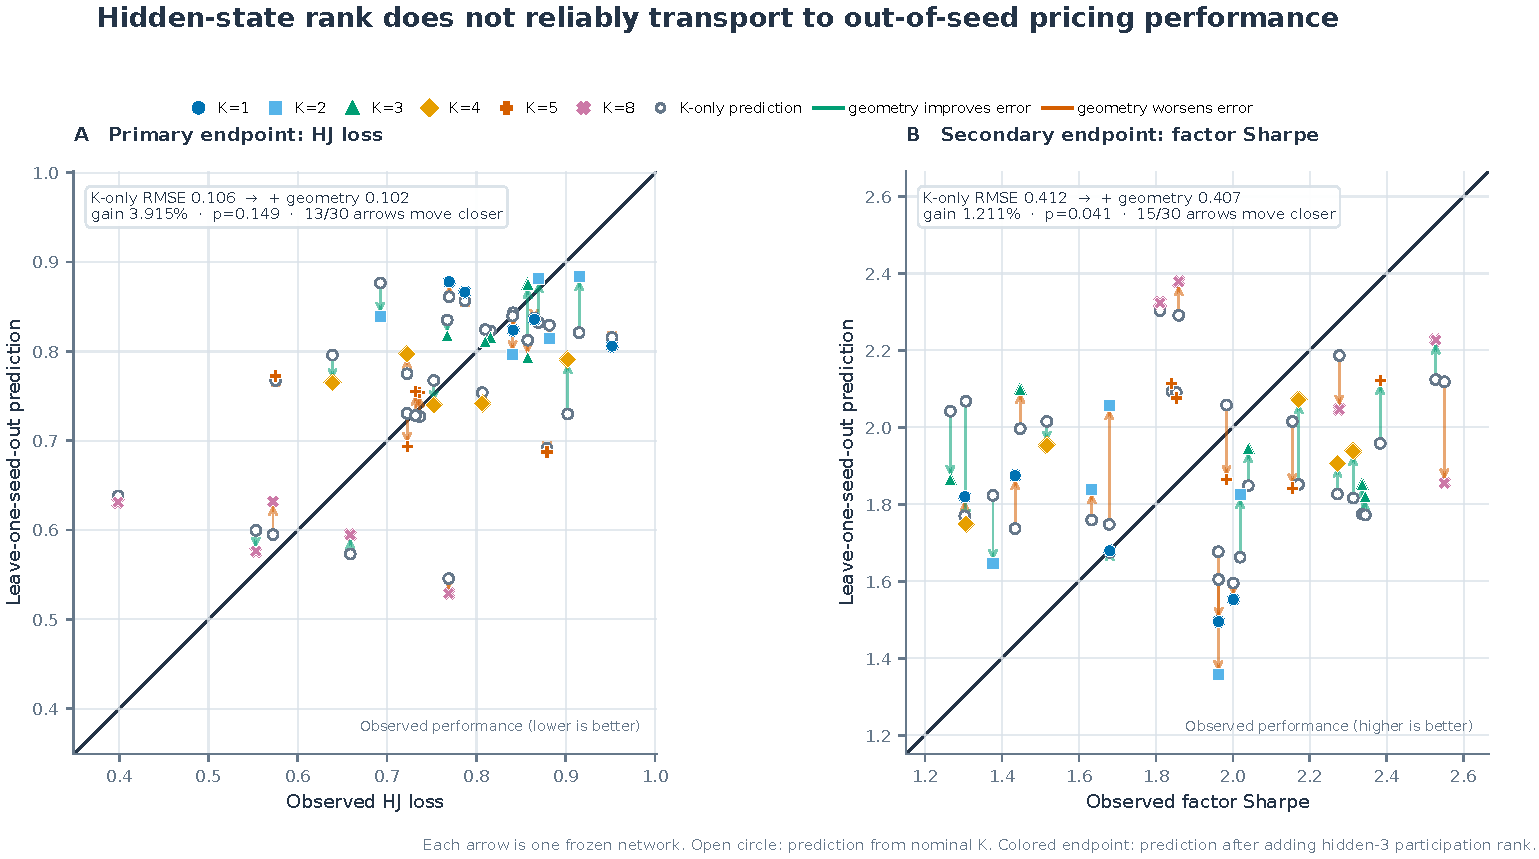
\includegraphics[width=0.98\textwidth]{figure_01_evidence_ladder.pdf}
\caption{Leave-one-seed-out pricing predictions with and without hidden-state geometry. Each arrow is one of 30 frozen Core-86 diagnostic networks, not a model from the later conditional-autoencoder extension. Open circles use nominal factor count alone; colored endpoints add hidden-3 raw-centered participation rank, with color and shape identifying nominal $K$. Arrows ending closer to the 45-degree line improve prediction. Geometry reduces HJ-loss RMSE by 3.915\%, below the prespecified 5\% gate ($p=0.149$), and reduces factor-Sharpe RMSE by only 1.211\%. The figure displays the prediction errors behind those aggregate gates rather than rescaled diagnostic ranks. Plotting code was developed with OpenAI Codex assistance; the visualization is computed from archived data.}
\label{fig:evidence-ladder}
\end{widefigure}

\subsection{Why minimum validation loss need not select the minimal dimension}

We give an exact calculation for the known-loading Gaussian design used in Section~4. This is a result about a finite nested family of linear pricing spans, not a consistency theorem for independently trained neural networks.

Let $W$ be fixed and positive definite, and let $P_K$ be the $W$-orthogonal projector onto the span of the first $K$ columns of a full-column-rank loading matrix. The candidate set is finite and contains the smallest correct dimension $K_0$, with $P_{K_0}\mu=\mu$. Independent training and evaluation means satisfy
\begin{equation}
 \bar R_n=\mu+n^{-1/2}U,\qquad
 \bar R_T^{e}=\mu+T^{-1/2}V,
\end{equation}
where $U,V$ are independent $N(0,\Sigma)$ and $\Sigma$ is positive definite. Fit $\widehat\mu_K=P_K\bar R_n$ and evaluate
\begin{equation}
 \widehat\Loss_T(K)=\|\bar R_T^{e}-\widehat\mu_K\|_W^2,
 \qquad \|x\|_W^2=x'Wx.
\end{equation}
For $K>K_0$, put $Q_K=P_K-P_{K_0}$. Orthogonality gives the exact identity
\begin{equation}
 T\{\widehat\Loss_T(K)-\widehat\Loss_T(K_0)\}
 =\frac{T}{n}\|Q_KU\|_W^2
 -2\sqrt{\frac{T}{n}}V'WQ_KU.
 \label{eq:nondegenerate-diff}
\end{equation}

\begin{proposition}[Raw validation selection in the known-loading design]
\label{prop:inconsistency}
Suppose $n/T\to c\in(0,\infty)$ and the candidate set includes at least one $K>K_0$. If every smaller candidate has $\|(I-P_K)\mu\|_W^2>0$, under-selection vanishes but the probability that the unpenalized validation minimizer differs from $K_0$ stays bounded away from zero.
\end{proposition}

Conditional on $U$, the second term in Eq.~\eqref{eq:nondegenerate-diff} is a nondegenerate normal variable whenever $Q_KU\ne0$, an event of probability one. It therefore exceeds the first term with positive probability. An overfitted candidate then beats $K_0$, even as the unscaled loss difference converges to zero. Underfitted candidates instead retain a fixed positive population gap. Supplement~A gives the full argument.

\begin{corollary}[A sufficient penalty rate in this design]
\label{cor:penalty}
For the same finite candidate family, minimizing $\widehat\Loss_T(K)+p_TK$ consistently selects $K_0$ if $p_T\to0$ and $Tp_T\to\infty$.
\end{corollary}

The penalty dominates every $O_p(T^{-1})$ overfit difference while remaining smaller than each fixed underfit gap. With oracle evaluation of the population mean, the cross term in Eq.~\eqref{eq:nondegenerate-diff} is absent and an overfitted candidate cannot improve on $K_0$. Thus the simulation isolates evaluation noise without estimating loadings or the covariance matrix. An estimated weight matrix, different training-to-validation ratio, growing candidate set, or nonlinear fitted family requires a separate analysis. The penalty result is a theoretical benchmark; this paper does not report an empirical comparison of penalty choices.

\section{Data and frozen empirical design}

\subsection{U.S. equity panel and information timing}

The reconstructed stock panel uses CRSP CIZ daily stock data aggregated to calendar months, Compustat North America annual and quarterly records, and CCM link history. It is not a direct extract of the CRSP Monthly Stock File. Monthly returns compound daily total returns after duplicate distribution rows are resolved; the CIZ delisting return is retained rather than added again. The pipeline keeps the frozen common-stock classification and date-valid accounting links. Annual accounts use a six-month lag; quarterly availability uses the recorded reporting date when admissible and a conservative fallback otherwise. These rules limit timing errors but do not turn a current-vintage accounting database into a point-in-time vintage archive.

The reconstructed panel spans 1950--2025. The Core-86 training period contains 437 target-return months from August 1963 through December 1999. Validation and development contain 120 target months each, January 2000--December 2009 and January 2010--December 2019. Characteristic months precede target months by one. The later evaluation contains 72 target months, January 2020--December 2025, and 286,565 stock-month observations.

Core-86 contains 20 monthly/market, 10 quarterly, and 56 annual characteristics. The production input is a documented bridge: it retains nonmissing public benchmark characteristics where available through 2021 and uses audited self-built values otherwise. It is therefore not an entirely independent reconstruction of every historical value. Monthly cross-sectional ranks are mapped to $[-1,1]$; missing ranks are set to zero and accompanied by separate indicators. The 86 characteristics thus generate 172 network inputs. Relative to the earlier 92-characteristic non-announcement benchmark, the omitted columns are \texttt{ms}, \texttt{ps}, \texttt{tb}, \texttt{bm\_ia}, \texttt{chpmia}, and \texttt{pchcapx\_ia}. Supplement~B and the replication package give the variable dictionary and construction scripts.

A chronology limitation affects the legacy comparison. Core-92 used characteristic-month splits: its nominal 2010--2019 development block realizes returns in February 2010--January 2020, whereas Core-86 realizes returns in January 2010--December 2019. Consequently, Core-92/Core-86 differences combine feature membership, reconstruction and coverage, and a one-month shift in the evaluation window. They are a comparison of archived data pipelines, not an isolated six-feature deletion experiment. The overlap also means that January 2020 had entered legacy development before the later 2020--2025 evaluation was fixed. We call that exercise a \emph{locked later-period evaluation}, not a wholly untouched holdout for the research process. Its Core-86 weights and decision rules were fixed before that evaluation.

The analysis avoids corporate announcements, news text, analyst narratives, and language-model embeddings. The information set consists of market and accounting variables whose timing can be encoded as reproducible tabular data. This restriction isolates whether nonlinear pricing structure can be learned from conventional numerical information.

\subsection{Later same-panel feature control}

To isolate feature removal from the archived pipeline contrast, a later paired experiment starts from one Core-92 mother panel. It contains 2,068,593 training, 606,278 validation, and 444,538 development stock-months under the target-month calendar used by Core-86. Both arms load the same ordered rows, ranked values, missingness indicators, returns, and test-asset outcomes. All 184 input positions and hidden widths are retained. In the masked arm only, the six excluded characteristic columns and their six missingness indicators are set to zero. Each of the six $K$ values and five seeds receives the same initial parameter tensors in both arms; optimizer settings and the validation stopping rule are unchanged. This produces 30 pairs, or 60 additional models, without architecture or hyperparameter search.

The primary comparisons are all six fixed-$K$ paired pricing-distance differences for the combined 74 assets at geometry endpoints zero and one. Full curves for all three primary asset families, complete rankings, and winner margins are retained. A thousand common twelve-month circular-block draws resample development months and paired seed clusters while retaining every candidate. Validation SDF coefficients remain fixed; the evaluation return second moment and all losses are recomputed in each draw. Intervals are pointwise, conditional on trained models and validation estimates, and do not establish simultaneous coverage or a unique true $K$.

This experiment was designed after the original findings and initial replication release. Its specification was fixed before it ran, but the historical sample was already familiar. It is a post-study control, not fresh confirmation. It isolates information removal within the chosen panel and training procedure; it does not identify the contribution of coverage, accounting vintage, reconstruction, or timing to every historical pipeline difference.

\subsection{Original diagnostic neural family}

The original diagnostic family contains 30 neural pricing models. Nominal factor dimension is
\[
 K\in\{1,2,3,4,5,8\},
\]
and each dimension is estimated under five fixed random seeds, 20260924 through 20260928. All models within a data-definition exercise share the architecture, optimization rule, stopping rule, sample splits, and target construction. Dimension and seed are the planned sources of variation. Model selection uses the validation decade. The development decade and the locked period never alter weights or hyperparameters.

Each network has hidden widths 128, 64, and 32, SiLU activations, and a $K$-wide tanh output. Within a month, output scores are centered and normalized separately to unit gross exposure, producing zero-net-investment characteristic-managed factors. Training minimizes three times normalized ridge-HJ span loss minus 0.25 times the annualized factor-span Sharpe, plus 0.05 times squared off-diagonal factor correlations and 0.001 times portfolio concentration. Only the 25 size--book-to-market assets enter this training loss. AdamW uses learning rate $3\times10^{-4}$, weight decay $10^{-5}$, batches of 120 months, at most 80 epochs, and patience 12. Supplement~B specifies normalization and checkpoint selection.

This family was retained for diagnostics after earlier benchmark-advancement criteria failed. It should not be interpreted as a demonstrated state-of-the-art pricing model. Architecture is constant across $K$ apart from output width, but separately trained networks are not algebraically nested. The known-loading simulation removes optimization and separates this limitation from the statistical selection issue.

Random seeds are algorithmic repetitions. We summarize across them because a claimed economic dimension should not depend on one initialization, but we do not treat five seeds as five independent economic time series. Time-series uncertainty is obtained from the monthly sequence and the prespecified block bootstrap.

\subsection{Test assets and external transport}

The primary test assets are 25 size--book-to-market portfolios, 49 industry portfolios, and their 74-asset union. The two component sets emphasize different economic spans: characteristic-sorted portfolios organize the cross-section by size and valuation, while industries load on sector-specific cash-flow risks. The union is the main broad pricing panel.

Six external families test transport beyond the primary assets: 25 portfolios sorted on size and operating profitability, investment, momentum, accruals, market beta, and residual variance. These assets were fixed before the corresponding development and locked evaluations. They are useful because a direction that is weakly represented in size--value or industry portfolios can be more visible in an economically targeted family.

The locked exercise evaluates all nine sets: the three primary sets and six external sets. It does not add assets after observing 2020--2025 outcomes. Public portfolio returns and factor series can be independently obtained from the Kenneth French Data Library; stock-level model construction requires licensed CRSP and Compustat access.

\subsection{Pricing losses and the geometry path}

For each model, factor self-pricing coefficients are estimated in the validation block and then held fixed. Let $F$ be its validation factor matrix. The coefficient is $b=(F'F/T_v+\eta I)^{-1}\bar F$, with $\eta=10^{-6}\operatorname{tr}(F'F/T_v)/K$ and a numerical floor. Evaluation moments are $\hat g=T_e^{-1}\sum_t(1-b'F_t)R_t$. Alphas are intercepts from evaluation-period time-series regressions, a separate descriptive estimand.

Write the evaluation return second moment as $S=V\operatorname{diag}(\lambda_j)V'$. For $\gamma\in\{0,0.05,\ldots,1\}$, the actual geometry path is
\begin{align}
 d_j(\gamma)&=(\lambda_j+\epsilon)^{-\gamma},\\
 W_\gamma&=\frac{J\,V\operatorname{diag}(d_j(\gamma))V'}{\sum_jd_j(\gamma)\lambda_j},\\
 D_{K,s,A}(\gamma)&=\sqrt{12\hat g'W_\gamma\hat g},
\end{align}
where $\epsilon=10^{-4}\operatorname{tr}(S)/J$. This is a spectral-power path with $\operatorname{tr}(W_\gamma S)=J$, not a linear mixture of endpoint matrices. At zero it is a scaled equal-moment norm; at one it is a scaled regularized HJ-type norm. The displayed values are dimensionless annualized distances, not percentage returns. For these original diagnostic experiments, the evaluation second moment determines the metric; it is not an investor's ex-ante estimate of $W$. Coefficients $b$ remain fixed along the path. The later conditional-autoencoder extension instead fixes $W$ using validation returns, as specified in Section~\ref{sec:cae-control}. Distances from these two protocols are not pooled or interpreted as a common cross-experiment ranking.

The aggregate best dimension minimizes the seed-mean distance at each $\gamma$. We report the entire six-dimension ordering and seed-level winners in addition to the aggregate optimum. This matters because a common average winner can mask dispersion across training runs.

The market-direction diagnostic estimates each test asset's market beta in the validation decade, freezes that beta, and subtracts the associated market payoff in the development or locked period. Define $A_A=[\bar D_{1,A}(0)-\bar D_{5,A}(0)]-[\bar D_{1,A}(1)-\bar D_{5,A}(1)]$, where bars average the five seeds. Market attenuation is
\begin{equation}
 \Delta_A^{mkt}=|A_A|-|A_A^{hedged}|.
\end{equation}
A positive value means that removing the validation-estimated market direction makes the geometry contrast smaller. Betas are never re-estimated on the evaluation period.

The economic-completion diagnostic augments the one-factor neural representation with the observed market excess return. It evaluates both raw Euler moments and time-series alpha. Joint improvement is required because fitting a dominant unconditional moment can leave relative cross-sectional pricing errors unchanged.

\subsection{Development evidence and the locked later evaluation}

The development analysis maps the full geometry surface, compares Core-92 and Core-86, evaluates the six external families, decomposes spectral directions, and records the market-hedge diagnostics. It is discovery evidence: the sample informed the final hypotheses even though each underlying run used a frozen local protocol.

The later-period protocol was fixed after the development diagnostics. The January 2020 overlap described above prevents a claim of wholly untouched confirmation. The 30 Core-86 checkpoints were unchanged. Four hypotheses were fixed:
\begin{enumerate}
 \item the best dimension changes across endpoint geometries for the combined assets and for at least four of six external families;
 \item removing the frozen market-beta direction attenuates geometry sensitivity for the combined assets and at least four external families;
 \item adding the market factor to $K=1$ jointly improves raw moments and alpha for at least four external families; and
 \item external families select at least three distinct best dimensions across the endpoints.
\end{enumerate}
The run uses 500 twelve-month circular block-bootstrap draws. Point-estimate gates and confidence intervals are both reported; passing a directional point-estimate rule does not convert an interval that crosses zero into precise evidence.

\subsection{Known-truth identification simulation}

The simulation asks whether the observed instability can arise even when the true dimension is known and neural optimization is absent. It contains 500 Monte Carlo replications for each of 144 base conditions. The design crosses true dimensions $K_0\in\{1,3,5\}$, sample lengths $T\in\{72,240,600\}$, strong and weak risk prices, full and weak-tail asset spanning, factor correlation $\rho\in\{0,0.7\}$, and 25 versus 74 test assets. Six independently drawn asset families and two pricing geometries are evaluated.

The candidate dimensions contain the truth. Both modes estimate risk prices from a noisy training mean. Oracle evaluation compares the fitted mean with the population mean; feasible evaluation compares it with an independent noisy mean of the same sample length. Both modes know the loading matrix and population covariance; ``feasible'' here refers only to evaluation-mean noise. The HJ-labelled simulation weight uses a regularized covariance, whereas the empirical path uses return second moments. This is a mechanism experiment, not a literal replication of the empirical estimator. Because true loadings are provided, any difference between oracle and feasible recovery is attributable to dimension identification and evaluation noise rather than a network failing to optimize.

The simulation was frozen before execution. It generated 576 condition summaries, 3,456 selection-frequency rows, and 864 cross-asset disagreement summaries. A second run using the same code and seeds reproduced all four output files byte for byte. Eight directional mechanism tests were fixed in advance: improvements with sample length, strong prices, and complete spanning; greater under-selection under weak prices; greater cross-asset disagreement with weak-tail spanning; disagreement across geometries; amplification of that disagreement with correlation or weak spanning; and better recovery under oracle evaluation.

\subsection{Scope of the separate temporal replay}

Supplement~D documents a retrospective return-prediction replay with neural, Ridge, and shallow-tree estimators. It is not a refit of the 30 pricing-dimension networks. The stock universe and historical model choices are selected using overlapping research history. Its results are retained as a boundary case for economic-use claims, not a prospective investability test or evidence that latent pricing dimension changes. The numerical results and full implementation remain in the supplement.

\subsection{Hidden-representation geometry}

The geometry sample contains the same 30 frozen Core-86 networks, 120 development months, 384 securities per month, 172 inputs (86 ranked characteristics and 86 missingness indicators), and three hidden layers. For every model, month, and layer we calculate participation rank, entropy rank, PCA90 and PCA95 dimension, and a collapse indicator. Neighbor-based TWO-NN and Levina--Bickel ($k=20$) dimensions and a tangent-angle diagnostic are computed only every twelfth development month (ten months) under raw centering and feature z-scoring. They are not computed under row normalization. We repeat the spectral statistics under raw centering, feature z-scoring, and row-$L_2$ normalization.

Because layer widths differ, we additionally report participation rank divided by width and the later architecture-matched random-network control in Section~\ref{sec:geometry}. Its protocol was fixed before that control ran, after the earlier results had been inspected. It does not create an independent confirmation sample.

CKA measures adjacent-layer similarity. Rank-five principal-subspace Grassmann distance measures month-to-month drift. The primary functional probe asks whether hidden geometry improves leave-one-seed-out prediction of development-period HJ loss after controlling for nominal factor count. Advancement requires at least a 5\% RMSE reduction and a within-factor-count permutation $p\leq0.05$. The factor-Sharpe probe is secondary and cannot replace the primary endpoint.

\subsection{Conditional-autoencoder extension and inference calibration}

The later extension uses the first 92 ranked characteristics of the common mother panel, without missingness indicators. It retains the same target-month training, validation, and development calendars and contains 2,068,593, 606,278, and 444,538 stock-months, respectively. Its linear-loading and nonlinear-loading arms are distinct from the original score-based pricing networks. Nonlinear loadings have hidden widths 32, 16, and 8. Factors are encoded linearly from the constant and 92 ridge characteristic-managed portfolios. Reconstruction loss, rather than the original pricing objective, fits the model. Each architecture and $K$ has five seeds and two $L_1$ settings ($10^{-6}$ and $10^{-4}$); Adam uses learning rate 0.001, at most 60 epochs, patience eight, and batches of 24 months. Validation reconstruction loss selects regularization and epoch separately for each architecture, $K$, and seed. The frozen protocol is P1-G4-V003.

The primary comparison uses the combined 74 assets with validation-estimated SDF coefficients and a fixed validation-estimated pricing weight.
For the audited secondary surface, let $S_v=R_v^{\top}R_v/T_v=U\operatorname{diag}(\lambda_i)U^{\top}$ be the uncentred validation return second moment for the relevant asset family. The implemented ridge is $\eta=10^{-4}\max\{\operatorname{tr}(S_v)/N,10^{-12}\}$, and
\begin{equation}
 a_i=(\max\{\lambda_i,0\}+\eta)^{-\gamma},\qquad
 W_{v,\gamma}=U\operatorname{diag}\!\left(\frac{N a_i}{\sum_j\lambda_j a_j}\right)U^{\top}.
\end{equation}
For seed $s$, $D_{s,\gamma}=\sqrt{12\bar g_s^{\top}W_{v,\gamma}\bar g_s}$, where $\bar g_s=T^{-1}\sum_t m_{s,t}R_t$. Each reported candidate mean is $5^{-1}\sum_s D_{s,\gamma}$; it is not the norm of averaged seed moments. The same validation-fitted SDF coefficients are used for all three asset families and five weights. Thus the within-architecture comparison changes the evaluation task without refitting the network or SDF. These secondary-surface weights are not the evaluation-fitted weights of the legacy diagnostic family.
 The exploratory uncertainty procedure uses 1,999 common twelve-month circular-block and seed-resampling draws, without refitting networks or validation coefficients. A separate moment-level simulation, P1-G4-V004, evaluates its 15 simultaneous within-autoencoder dimension intervals. It does not calibrate all other confidence intervals in this paper. The extension and calibration were specified after the original paper; neither turns the development decade into a new confirmatory sample. \ref{app:inference-calibration} reports the calibration failure and resulting limits.

\subsection{Evidence hierarchy and reproducibility}

We label evidence as descriptive, development, exploratory, or locked. ``Prespecified'' denotes a time-stamped local protocol fixed before its run, not registration in an external registry. The label determines permissible interpretation. Development findings motivate hypotheses. A locked failure remains a failure even when a related point estimate has the expected sign. Exploratory break dates cannot be presented as real-time rules. Secondary endpoints cannot rescue failed primary gates.

The project archives protocols, source hashes, model hashes, random seeds, manifests, execution receipts, and derived tables. Licensed raw CRSP and Compustat records cannot be redistributed, but the data dictionary, construction code, source links, and checksums document how licensed researchers can reconstruct the stock-level panel. Exact historical bytes require the same source vintages; current downloads can differ because of vendor revisions. All figures in this manuscript are produced from frozen CSV or JSON outputs; no value is transcribed from an unfrozen interactive analysis.

\section{Pricing dimension: empirical sensitivity and statistical identification}

\subsection{Development-period dimension surfaces}

Within the original diagnostic family, the preferred dimension changes with the data definition and pricing geometry (Figure~\ref{fig:dev-surfaces}). Each row is a candidate dimension within one feature-lineage--test-asset environment, and each column is one of the 21 evaluation geometries. Cell color measures the percentage pricing-distance loss relative to the pointwise best candidate, so the figure preserves both the winner and the economic size of every model's shortfall. The outlined path follows the winner based on the five-seed mean, while circle size records how many individual seeds select that row. A single model does not dominate every asset family and every geometry. For Core-86, the aggregate endpoint winner for the combined 74 assets moves from $K=2$ under the equal-moment endpoint to $K=4$ under the HJ endpoint. The industry and size--book-to-market sets move from $K=2$ to $K=1$. For Core-92, the equal-moment endpoint selects $K=5$ for all three primary sets, while the HJ endpoint selects $K=1$, $4$, and $8$ for the combined, industry, and size--book-to-market assets.

\begin{widefigure}[!tbp]
\centering
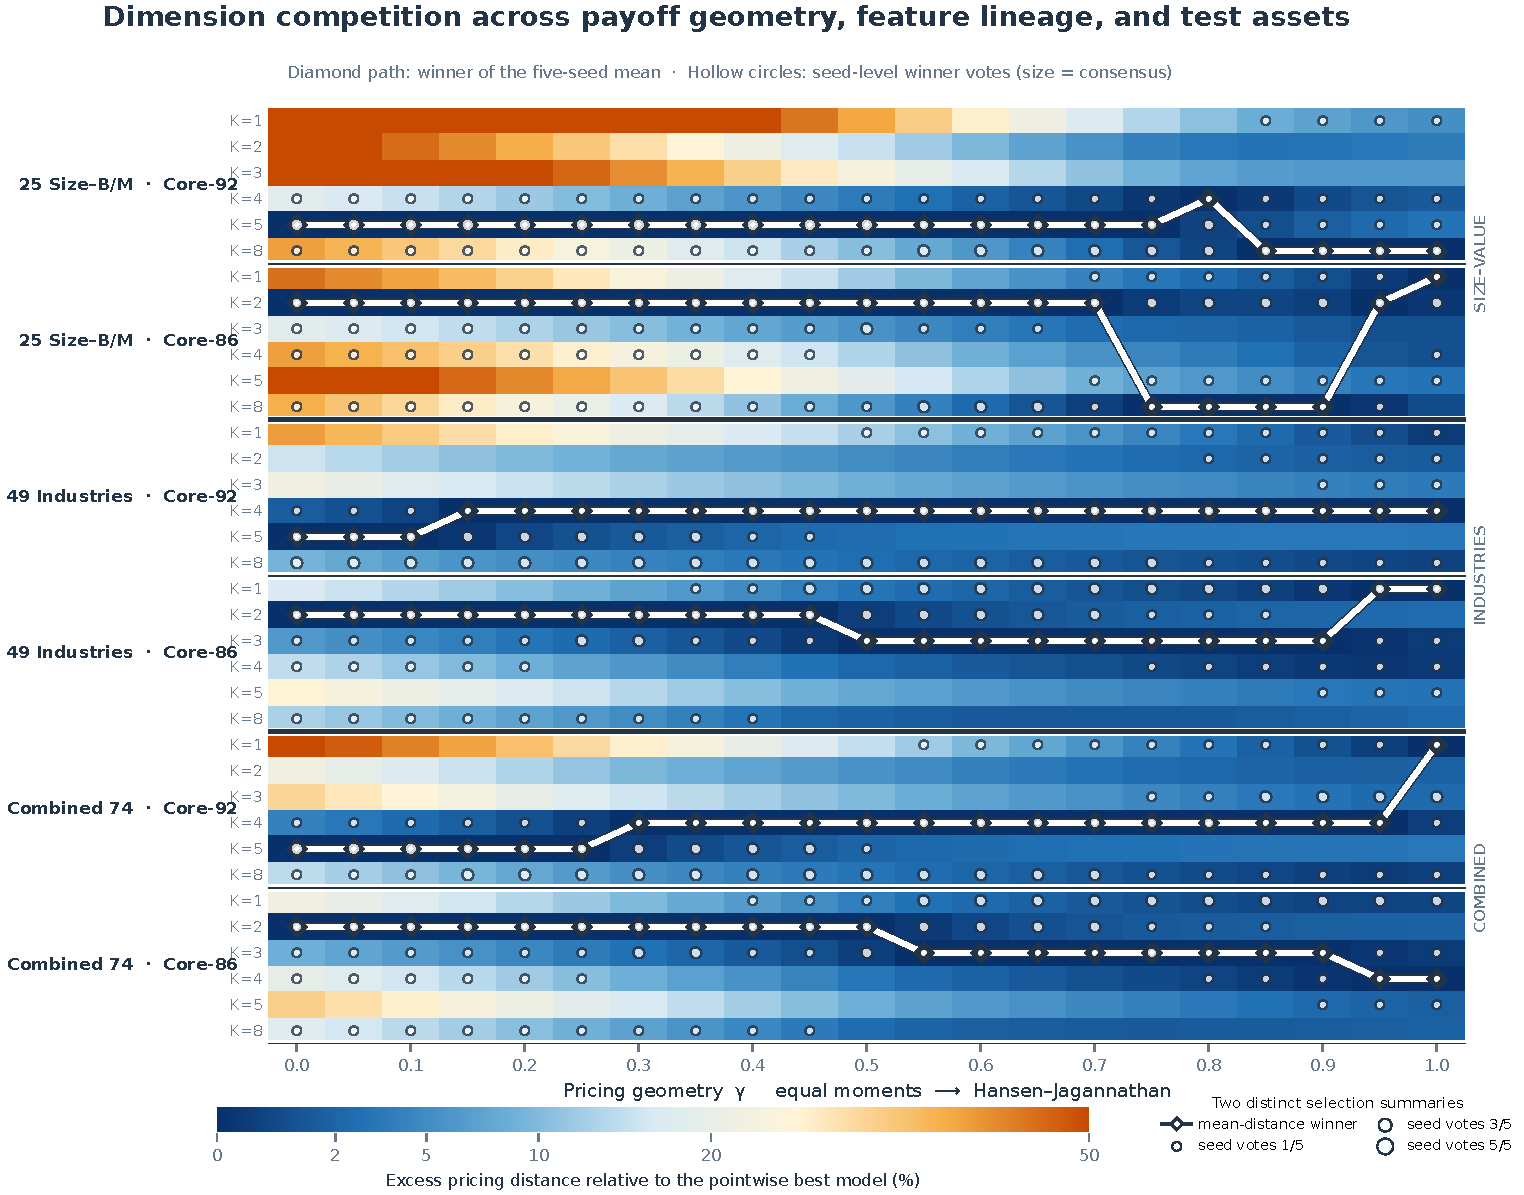
\includegraphics[width=0.98\textwidth]{figure_02_dimension_sensitivity.pdf}
\caption{Empirical dimension-competition field. The 756 cells report every frozen five-seed mean for the archived development windows: two characteristic definitions, three primary test-asset sets, six candidate dimensions, and 21 evaluation geometries. Color is excess pricing distance relative to the best candidate in the same environment and geometry, clipped at 50\% for display; dark blue denotes close competition and orange denotes economically large shortfall. The outlined diamond path follows the winner of the five-seed mean. Hollow circles are a distinct statistic: their area records one to five seed-level winner votes for the corresponding dimension, computed from all 3,780 seed-specific distances. A circle away from the diamond path therefore indicates seed-level support that does not win after averaging. Geometry zero is the equal-moment endpoint and one is the HJ-type endpoint. Core-92 evaluates February 2010--January 2020 returns; Core-86 evaluates January 2010--December 2019 returns. The comparison also changes construction and coverage, not only feature count. Plotting code was developed with OpenAI Codex assistance; the visualization is computed from archived data.}
\label{fig:dev-surfaces}
\end{widefigure}

Table~\ref{tab:dimension-evidence} reports all six candidate dimensions at both endpoints. Its common column structure allows a direct comparison of Core-92 and Core-86 within each asset set. Boldface identifies the seed-mean minimum; neighboring entries show whether that minimum is separated from the alternatives. Parentheses summarize dispersion across five fixed training seeds, not time-series sampling uncertainty.

\begin{widetable}[!tbp]
\centering
\begin{minipage}{\textwidth}
\caption{Pricing distances for every candidate dimension, archived development windows}
\label{tab:dimension-evidence}
\footnotesize
\setlength{\tabcolsep}{4pt}
\renewcommand{\arraystretch}{1.16}
\begin{tabular*}{\linewidth}{@{\extracolsep{\fill}}crrrr@{}}
\toprule
 & \multicolumn{2}{c}{Core-92} & \multicolumn{2}{c}{Core-86} \\
\cmidrule(lr){2-3}\cmidrule(l){4-5}
$K$ & Equal moments & HJ & Equal moments & HJ \\
\midrule
\multicolumn{5}{@{}l}{\textit{A. 25 size--book-to-market portfolios}} \\[2pt]
$1$ & 3.321 (0.183) & 1.840 (0.022) & 2.365 (0.105) & \textbf{1.841} (0.038) \\
$2$ & 2.455 (0.219) & 1.809 (0.036) & \textbf{1.633} (0.143) & 1.843 (0.037) \\
$3$ & 2.725 (0.306) & 1.856 (0.070) & 1.935 (0.167) & 1.858 (0.024) \\
$4$ & 1.893 (0.205) & 1.771 (0.050) & 2.269 (0.391) & 1.857 (0.024) \\
$5$ & \textbf{1.597} (0.314) & 1.798 (0.041) & 2.564 (0.315) & 1.895 (0.054) \\
$8$ & 2.221 (0.336) & \textbf{1.746} (0.047) & 2.236 (0.325) & 1.854 (0.023) \\
\addlinespace[5pt]
\multicolumn{5}{@{}l}{\textit{B. 49 industry portfolios}} \\[2pt]
$1$ & 4.305 (0.126) & 2.332 (0.030) & 3.465 (0.137) & \textbf{2.306} (0.054) \\
$2$ & 3.566 (0.201) & 2.363 (0.048) & \textbf{2.964} (0.130) & 2.365 (0.042) \\
$3$ & 3.771 (0.326) & 2.411 (0.080) & 3.151 (0.117) & 2.311 (0.061) \\
$4$ & 3.137 (0.217) & \textbf{2.328} (0.041) & 3.394 (0.276) & 2.310 (0.044) \\
$5$ & \textbf{3.088} (0.207) & 2.403 (0.041) & 3.718 (0.251) & 2.376 (0.084) \\
$8$ & 3.371 (0.285) & 2.337 (0.041) & 3.348 (0.212) & 2.360 (0.061) \\
\addlinespace[5pt]
\multicolumn{5}{@{}l}{\textit{C. Combined 74 portfolios}} \\[2pt]
$1$ & 5.410 (0.199) & \textbf{2.802} (0.025) & 4.208 (0.168) & 2.750 (0.041) \\
$2$ & 4.343 (0.277) & 2.854 (0.042) & \textbf{3.438} (0.177) & 2.790 (0.033) \\
$3$ & 4.651 (0.433) & 2.867 (0.073) & 3.735 (0.177) & 2.743 (0.055) \\
$4$ & 3.706 (0.277) & 2.808 (0.034) & 4.115 (0.421) & \textbf{2.738} (0.032) \\
$5$ & \textbf{3.559} (0.308) & 2.895 (0.033) & 4.535 (0.362) & 2.785 (0.069) \\
$8$ & 4.067 (0.403) & 2.811 (0.035) & 4.058 (0.324) & 2.788 (0.049) \\
\bottomrule
\end{tabular*}
\par\vspace{4pt}
{\footnotesize\raggedright\textit{Notes:} Each entry is a mean pricing distance over five fixed training seeds; parentheses give the standard error across seeds. Lower is better. Boldface marks the smallest mean within each asset set, data definition, and loss geometry. Seed standard errors describe algorithmic dispersion, not time-series sampling uncertainty. Core-92 return months are February 2010--January 2020; Core-86 return months are January 2010--December 2019. Construction and coverage also differ. All six candidates are shown, including those that never win.\par}
\end{minipage}
\end{widetable}


The result is not merely that two losses produce two answers. The economic content of a pricing error depends on direction. Equal weighting emphasizes the coordinate representation of the moments. HJ weighting discounts directions with large payoff second moments and emphasizes directions that are expensive to span. If weak priced directions are correlated with dominant common directions, a change in $W$ changes the signal-to-noise tradeoff. A dimension claim that is robust only to one geometry is therefore a statement about that loss, not a loss-free risk count.

\subsection{How costly is a different dimension?}
For a fixed pipeline, asset family and target endpoint $g$, let $D_g(K)$ be the archived mean pricing norm and let $\widehat K_g$ minimize it. We report the retrospective transfer cost
\begin{equation}
 C_{h\to g}=D_g(\widehat K_h)-D_g(\widehat K_g),\qquad
 C_{h\to g}^{\mathrm{rel}}=100 C_{h\to g}/D_g(\widehat K_g).
\end{equation}
The same target loss evaluates both candidates. The other endpoint chooses the transferred dimension on the same historical development sample. This is a descriptive audit of objective dependence, not an out-of-sample model-selection rule or an estimate of regret relative to the true economic dimension.

\begin{widetable}[!tbp]
\centering\small
\caption{Cost of transferring the preferred dimension between evaluation endpoints}
\label{tab:transfer-cost}
\begin{tabular}{llrrrrr}
\toprule Pipeline & Assets & Target $\gamma$ & Best $K$ & Transfer $K$ & Excess norm & Excess (\%) \\
\midrule
Core-86 & Combined 74 & 0 & 2 & 4 & 0.677 & 19.68 \\
Core-86 & Combined 74 & 1 & 4 & 2 & 0.053 & 1.93 \\
Core-86 & Industries & 0 & 2 & 1 & 0.501 & 16.89 \\
Core-86 & Industries & 1 & 1 & 2 & 0.059 & 2.55 \\
Core-86 & Size--B/M & 0 & 2 & 1 & 0.732 & 44.83 \\
Core-86 & Size--B/M & 1 & 1 & 2 & 0.002 & 0.11 \\
Core-92 & Combined 74 & 0 & 5 & 1 & 1.852 & 52.03 \\
Core-92 & Combined 74 & 1 & 1 & 5 & 0.093 & 3.33 \\
Core-92 & Industries & 0 & 5 & 4 & 0.049 & 1.57 \\
Core-92 & Industries & 1 & 4 & 5 & 0.075 & 3.24 \\
Core-92 & Size--B/M & 0 & 5 & 8 & 0.624 & 39.08 \\
Core-92 & Size--B/M & 1 & 8 & 5 & 0.052 & 2.97 \\
\bottomrule\end{tabular}
\par\smallskip\begin{minipage}{0.97\textwidth}\footnotesize Notes: Direct arithmetic from archived five-seed mean distances. Transfer $K$ is the dimension minimizing the other endpoint on the same development window; its cost is evaluated under the target endpoint. These are retrospective in-sample-to-evaluation-design comparisons, not a validation-selected trading policy. Excess is a pricing-norm difference; percentages are relative to the target sample minimum, not returns, welfare losses or true-dimension errors. No significance or equivalence claim is made. The two pipelines have different coverage and return windows and are not pooled.\end{minipage}
\end{widetable}


For Core-86 combined assets, transferring the HJ-preferred $K=4$ to equal moments adds 0.677 units (19.7\%) to the pricing norm; transferring the equal-moment-preferred $K=2$ to HJ adds 0.052 units (1.9\%). For Core-92 combined assets, the corresponding directions cost 1.852 units (52.0\%) and 0.093 units (3.3\%). Thus a change in the selected number need not imply a symmetric performance penalty. These percentages describe norm differences; they are not percentage-point return losses, statistical significance statements, or comparable welfare quantities across geometries.

\subsection{Data-definition and seed instability}

The archived Core-92 and Core-86 row blocks in Figure~\ref{fig:dev-surfaces}, together with Table~\ref{tab:dimension-evidence}, compare the entire six-dimension ordering under the two feature lineages. Exact agreement is nearly absent. Across 21 geometries, the best $K$ agrees twice for the 25 size--book-to-market portfolios, never for industries, and once for the combined assets. Mean Spearman correlations are $-0.355$, $-0.156$, and $-0.151$, respectively; their minima are $-0.600$, $-0.371$, and $-0.371$. Mean Kendall correlations are $-0.263$, $-0.111$, and $-0.124$. The color field also shows that the result is not uniformly driven by economically negligible ties: some switches occur within a broad blue region of small descriptive loss gaps, while others coincide with large orange shortfalls for the displaced candidate. Thus the change reaches beyond a close tie at the minimum; it reverses much of the ordering.

This archived comparison cannot separate feature information from measurement, coverage, missingness, and timing. We therefore retain it as a pipeline sensitivity result and examine deletion separately using the later same-panel control. Neither comparison identifies the marginal causal effect of an individual characteristic on expected returns.

Seed sensitivity points in the same direction. There are 12 combinations of data definition, primary asset set, and endpoint geometry. None yields a five-of-five unanimous best dimension. Averaging across seeds is a useful performance summary, but it does not make the underlying structural object seed-invariant. The distinction is analogous to model averaging: aggregation can stabilize a prediction while leaving model selection uncertain.

\subsection{What survives a same-panel feature ablation?}

The controlled comparison is less disruptive than the archived pipeline contrast. Keeping rows, return months, ranks, input positions, and paired initialization fixed produces mean rank correlations of 0.649 for size--book-to-market portfolios, 0.722 for industries, and 0.703 for the combined assets across the 21 geometries. Winner agreement occurs in 9, 9, and 11 geometries, respectively. Thus some exact minima still switch, but deleting the six features alone does not reproduce the broad negative rank correlations of the two archived pipelines in this design.

For the combined 74 assets, both full and masked arms select $K=4$ under equal moments and $K=5$ under the HJ-type endpoint. Table~\ref{tab:matched-features} retains all fixed-$K$ comparisons rather than reporting only those winners. Under the HJ-type endpoint the $K=5$ distance is 2.700 with all features and 2.699 after masking, a difference of $-0.0007$ with interval $[-0.0600,0.0700]$. All six HJ-endpoint paired intervals include zero. Under equal moments, masking raises the $K=1$ distance by 0.3855 with pointwise interval $[0.0172,0.9277]$; the remaining five intervals include zero. This single exclusion of zero among twelve primary intervals is not familywise evidence of a general feature effect.

\begin{widetable}[!tbp]
\centering
\begin{minipage}{\textwidth}
\caption{Matched six-feature ablation: pricing distances and paired uncertainty}
\label{tab:matched-features}
\footnotesize
\setlength{\tabcolsep}{4pt}
\renewcommand{\arraystretch}{1.16}
\begin{tabular*}{\linewidth}{@{\extracolsep{\fill}}crrrrc@{}}
\toprule
$K$ & Full 92 & Masked 86 & Difference & 95\% interval & $K^*$ frequency \\
\midrule
\multicolumn{6}{@{}l}{\textit{A. Equal-moment endpoint}} \\[2pt]
1 & 5.227 & 5.612 & +0.385 & [0.017, 0.928] & 0.0 / 0.0 \\
2 & 4.449 & 3.980 & -0.469 & [-1.280, 0.493] & 7.2 / 20.7 \\
3 & 4.257 & 3.900 & -0.358 & [-1.568, 0.600] & 16.3 / 19.7 \\
4 & 3.745 & 3.852 & +0.106 & [-0.612, 0.588] & 54.4 / 16.7 \\
5 & 4.106 & 3.994 & -0.111 & [-0.689, 0.466] & 20.0 / 30.6 \\
8 & 4.838 & 4.194 & -0.644 & [-2.066, 0.640] & 2.1 / 12.3 \\
\addlinespace[5pt]
\multicolumn{6}{@{}l}{\textit{B. HJ-type endpoint}} \\[2pt]
1 & 2.742 & 2.777 & +0.036 & [-0.031, 0.117] & 8.4 / 10.7 \\
2 & 2.715 & 2.763 & +0.048 & [-0.045, 0.184] & 29.2 / 10.3 \\
3 & 2.786 & 2.746 & -0.039 & [-0.169, 0.124] & 1.5 / 7.4 \\
4 & 2.753 & 2.787 & +0.034 & [-0.066, 0.180] & 1.5 / 6.7 \\
5 & 2.700 & 2.699 & -0.001 & [-0.060, 0.070] & 47.6 / 56.7 \\
8 & 2.739 & 2.813 & +0.073 & [-0.096, 0.299] & 11.8 / 8.2 \\
\bottomrule
\end{tabular*}
\par\vspace{4pt}
{\footnotesize\raggedright\textit{Notes:} Combined 74 assets, January 2010--December 2019. Distances average five seeds; difference is masked minus full, so positive values favor retaining all features. Both arms use the same mother panel, ordered stock-month rows, ranks, target-month clock, and paired initial weights. The six characteristic columns and their missingness flags are zeroed only in the masked arm. Intervals use 1,000 common twelve-month block draws with paired seed resampling and fixed validation coefficients; the evaluation second moment is re-estimated within each draw. These are pointwise intervals conditional on fitted models. $K^*$ frequency lists full/masked bootstrap winner percentages, not posterior probabilities of a true dimension.\par}
\end{minipage}
\end{widetable}


Figure~\ref{fig:matched-features} shows the complete combined-asset ablation paths. The direction and magnitude vary across candidate dimensions and seeds. Even unchanged winners can conceal different separation: at the equal-moment endpoint the first-to-second gap falls from 0.3603 in the full arm to 0.0481 in the masked arm. Exact selection therefore discards information about competition among neighboring candidates. Bootstrap winner frequencies in the table describe this conditional instability; they are not probabilities that a candidate is the economy's true risk dimension.

\begin{widefigure}[!tbp]
\centering
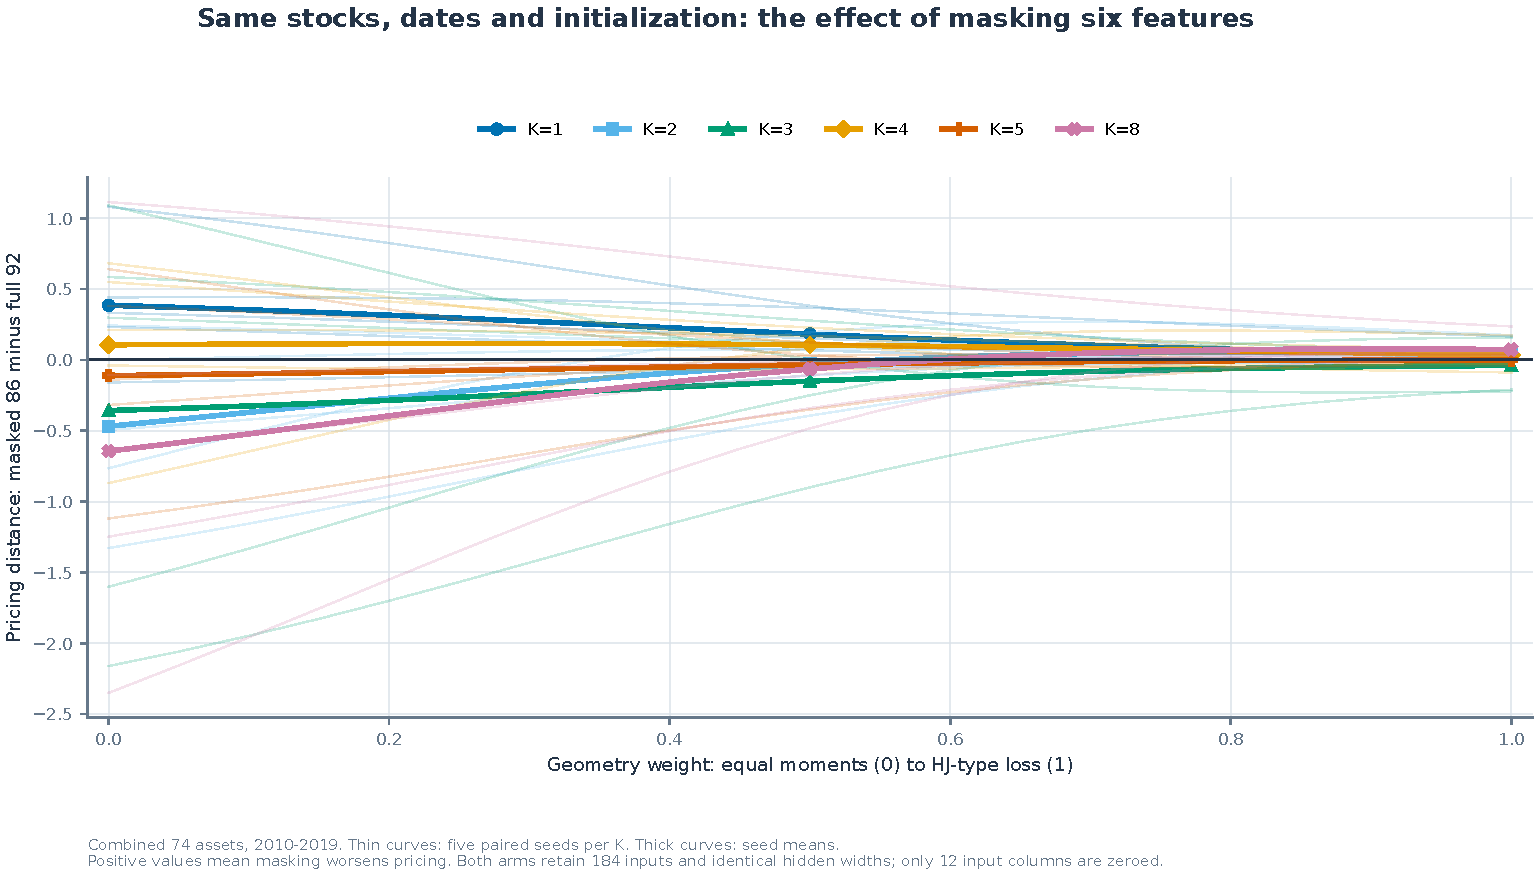
\includegraphics[width=0.98\textwidth]{figure_08_matched_feature_control.pdf}
\caption{Same-panel six-feature ablation for the combined 74 assets. Every curve is a paired difference, masked minus full, on the same 2010--2019 target-return months. Thin lines show all five paired seeds for each fixed $K$; thick lines show their means over the 21 prespecified geometry weights. Positive values mean that masking worsens pricing distance. Both arms have 184 input positions and 128--64--32 hidden widths; only the six characteristic columns and their six missingness indicators are zeroed in the masked arm. The endpoint block-bootstrap intervals are in Table~\ref{tab:matched-features}; thin-line dispersion is algorithmic variation, not a confidence band. Plotting code was developed with OpenAI Codex assistance; the visualization is computed from archived data.}
\label{fig:matched-features}
\end{widefigure}

The control changes the attribution, not the original archived numbers. The historical pipeline reversal cannot be read as a six-characteristic effect. Reconstruction, coverage, timing, and the different input parameterization remain bundled in that older comparison. The present experiment does not decompose their contributions. Its narrower result is that the information deletion tested here leaves endpoint winners for the combined assets unchanged while affecting candidate margins and some intermediate rankings. Geometry dependence persists within both matched arms, without identifying a structural risk count.

% IREF working fragment, 2026-10-06. Not a standalone submission manuscript.
% Sources: P1-G4-V003-R001; calibration qualification P1-G4-V004-R001.
\subsection{Conditional-autoencoder control and the interpretation of dimension}
\label{sec:cae-control}

To assess whether the earlier diagnostic findings extend to a model with more
favorable benchmark performance, we added a conditional-autoencoder control and
a matched linear-loading arm. This extension was specified after the original
study and uses familiar historical data; it is exploratory. The models use 92
ranked characteristics and candidate factor counts $K\in\{1,2,3,4,5,8\}$.
The training, validation, and development periods are August 1963--December 1999,
2000--2009, and 2010--2019, respectively. The extension does not access 2020--2025.
For each architecture, factor count, and initialization, validation reconstruction
loss selects the epoch and one of two regularization settings. Five initializations
produce 120 candidate fits and 60 selected models across the two architectures.
This is a conditional-autoencoder benchmark implementation, not an exact
replication of a published model.

The forecasting exercise uses fixed estimated loadings and expanding factor means
formed from strictly earlier observations. Contemporaneous factors are used for
reconstruction and pricing evaluation, not for forecasting the same month's
returns. SDF coefficients and regularized pricing weights are estimated using
validation data and held fixed in the development evaluation. The reported
pricing norm is HJ-type: it uses the study's regularization and normalization,
so its numerical scale should not be compared directly with differently
normalized HJ distances in other studies.

Validation predictive $R^2$ selects $K=8$ for the conditional autoencoder. Its
validation predictive $R^2$ is 0.0781\%, and its development predictive $R^2$ is
0.2687\%. Its development pricing distance on the combined 74-asset set is
5.0254, compared with 5.9582 for FF5 plus momentum. These point estimates satisfy
the prespecified diagnostic criteria of positive predictive $R^2$ in both periods
and a development pricing distance no larger than the reference. They do not
constitute a statistical noninferiority test or establish superiority over either
the reference factors or the matched linear-loading arm.

Table~\ref{tab:cae-candidates} retains every candidate in both arms. At $K=8$, the linear-loading model has development predictive $R^2$ of 0.2963\%, slightly above the conditional autoencoder, while its pricing distance is 5.1674. These different orderings preclude a general claim of nonlinear-model dominance.

\begin{widetable}[!tbp]
\centering
\caption{Conditional-autoencoder extension: complete development-period candidate comparison}
\label{tab:cae-candidates}
\small
\begin{threeparttable}
\noindent\resizebox{0.98\textwidth}{!}{%
\begin{tabular}{@{}r rrr rrr@{}}
\toprule
& \multicolumn{3}{c}{Linear loadings} & \multicolumn{3}{c}{Conditional autoencoder} \\
\cmidrule(lr){2-4}\cmidrule(lr){5-7}
$K$ & Predictive $R^2$ & Pricing distance & Win frequency & Predictive $R^2$ & Pricing distance & Win frequency \\
& (\%) & & (\%) & (\%) & & (\%) \\
\midrule
1 & 0.1555 & 6.0417 & 6.40 & 0.1375 & 6.0127 & 2.05 \\
2 & 0.1594 & 6.3576 & 0.00 & 0.1973 & 6.0961 & 0.05 \\
3 & 0.2323 & 6.1573 & 0.05 & 0.2269 & 5.9433 & 3.95 \\
4 & 0.2880 & 5.3790 & 9.50 & 0.2327 & 5.9172 & 0.40 \\
5 & 0.2903 & 5.2380 & 34.32 & 0.2513 & 5.5869 & 6.35 \\
8 & 0.2963 & 5.1674 & 49.72 & 0.2687 & 5.0254 & 87.19 \\
\bottomrule
\end{tabular}}
\begin{tablenotes}[flushleft]\footnotesize
\item Development period: 2010--2019, 120 months and 444,538 stock-months. Pricing uses the combined 74 assets with validation-fixed weights and SDF coefficients. FF5 plus momentum has pricing distance 5.9582 under the same protocol. Each candidate aggregates five selected initializations. Win frequencies use 1,999 common time-block and seed-resampling draws within each architecture; they are descriptive frequencies, not structural-dimension probabilities. No confidence interval or significance ranking is asserted by this table. $K=8$ is the upper endpoint of the prespecified grid. Raw distances are not directly comparable with those from the earlier evaluation-weighted diagnostic protocol.
\end{tablenotes}
\end{threeparttable}
\end{widetable}


Dimension selection is comparatively concentrated in this extension. Under the
prespecified joint time-block and initialization resampling, $K=8$ attains the
smallest development pricing distance in 87.19\% of draws. This is a descriptive
frequency under that resampling procedure, not a probability that the economy
has eight priced shocks. Moreover, eight is the upper endpoint of the fixed
candidate grid. The result qualifies any general statement that these models
necessarily produce unstable dimension choices. It establishes neither a global
optimum over factor counts nor a structural factor dimension.

All 15 pairwise dimension intervals from the exploratory simultaneous procedure
include zero. We do not interpret this as evidence of equivalence or structural
nonidentification. A subsequent, bounded known-truth calibration of that procedure
found simultaneous coverage of 83.5\% and 87.0\%, below the nominal 95\%, in its two
primary 120-month equal-distance scenarios. \ref{app:inference-calibration}
reports the design and results. Accordingly, the intervals remain an archived
exploratory output rather than a calibrated confidence set for dimension.
The separate pointwise forecasting and benchmark-comparison intervals were not
validated by that calibration either; the extension's substantive comparison is
therefore limited to the reported point estimates and descriptive selection
behavior.

The control separates a model's observed performance from the interpretation of
its selected width. It supplies a case with favorable point-estimate diagnostics
and comparatively concentrated selection, alongside the earlier diagnostic
family. The combined evidence does not establish that successful pricing models
share an unstable economic structure. Rather, claims about economic dimension
require an identified economic object and evidence beyond the fitted width,
activation rank, or minimum of a finite candidate loss grid.

\paragraph{Descriptive cost within the fixed candidate grid.}
The archived conditional-autoencoder pricing norms are 6.0127, 6.0961, 5.9433, 5.9172, 5.5869 and 5.0254 for $K=1,2,3,4,5,8$. Relative to the development minimum at eight, the respective excesses are 19.65\%, 21.31\%, 18.27\%, 17.75\%, 11.17\% and zero. For linear loadings, five instead of eight adds only 1.37\%. These calculations are direct transformations of Table~\ref{tab:cae-candidates}, not new training or hypothesis tests. They show why the identity of a selected count and its loss cost should be reported separately. The failed interval calibration prevents a validated significance or equivalence conclusion. Eight remains a grid endpoint, not an estimated global optimum.

\paragraph{Audit across the complete archived asset--weight grid.}
We checked the 900 rows of the existing secondary surface against the original output checksums and recomputed both validation and development norms from saved factors and asset returns. All 1,800 distances agree to numerical precision (maximum absolute discrepancy $1.3\times10^{-12}$). The twelve combined-asset HJ means reproduce Table~\ref{tab:cae-candidates}. Aggregation follows the original evaluator: compute the annualized norm for each seed, then average the five norms. No new networks or resampling draws are introduced.

\begin{widetable}[!tbp]
\centering\footnotesize
\caption{Complete asset--weight audit of the archived conditional-autoencoder extension}
\label{tab:cae-surface-audit}
\begin{threeparttable}
\begin{tabular}{@{}lrrrrrrr@{}}
\toprule & & \multicolumn{3}{c}{Linear loadings} & \multicolumn{3}{c}{Conditional autoencoder} \\
\cmidrule(lr){3-5}\cmidrule(lr){6-8}
Assets & $\gamma$ & Best $K$ & Min. & $K=5$ excess & Best $K$ & Min. & $K=5$ excess \\
 & & & norm & (\%) & & norm & (\%) \\ \midrule
25 Size--B/M & 0 & 5 & 1.418 & 0.00 & 8 & 1.658 & 3.27 \\
 & 0.25 & 5 & 1.489 & 0.00 & 8 & 1.651 & 4.35 \\
 & 0.5 & 8 & 1.607 & 1.08 & 8 & 1.705 & 5.65 \\
 & 0.75 & 8 & 1.731 & 3.36 & 8 & 1.832 & 5.58 \\
 & 1 & 8 & 1.869 & 3.66 & 8 & 1.981 & 3.96 \\
\addlinespace[3pt]
49 industries & 0 & 4 & 2.206 & 1.10 & 8 & 2.523 & 2.35 \\
 & 0.25 & 5 & 2.232 & 0.00 & 8 & 2.417 & 4.02 \\
 & 0.5 & 8 & 2.224 & 0.92 & 8 & 2.327 & 6.05 \\
 & 0.75 & 8 & 2.233 & 2.02 & 8 & 2.287 & 8.22 \\
 & 1 & 8 & 2.282 & 2.54 & 8 & 2.301 & 10.34 \\
\addlinespace[3pt]
Combined 74 & 0 & 4 & 2.656 & 0.27 & 8 & 3.036 & 2.53 \\
 & 0.25 & 5 & 2.791 & 0.00 & 8 & 2.998 & 4.66 \\
 & 0.5 & 8 & 3.161 & 0.82 & 8 & 3.220 & 7.54 \\
 & 0.75 & 8 & 3.953 & 1.32 & 8 & 3.906 & 9.81 \\
 & 1 & 8 & 5.167 & 1.37 & 8 & 5.025 & 11.17 \\
\addlinespace[3pt]
\bottomrule\end{tabular}
\begin{tablenotes}[flushleft]\footnotesize
\item Each minimum is over six candidates, using the arithmetic mean of five seed-specific annualized pricing norms, not the norm of an averaged SDF. Development is 2010--2019 (120 months). Validation-fitted SDF coefficients and weights remain fixed. Weights vary over the five archived values only; $\gamma=0$ and $1$ denote equal-moment and HJ-type endpoints. Excess is $100[D(5)/\min_K D(K)-1]$, so zero means the five-factor candidate minimizes the observed norm. No new fitting, resampling, or significance test is performed. Minima are retrospective; eight is a grid boundary. Values across different asset--weight tasks are not a single common objective. Tasks share model fits, seeds and overlapping asset returns; fifteen tasks are not fifteen independent replications. The full 180 means, seed dispersion, and all 900 source rows are indexed in the audit materials.
\end{tablenotes}\end{threeparttable}
\end{widetable}


Table~\ref{tab:cae-surface-audit} extends the existing primary comparison to every archived secondary task. For the conditional autoencoder, $K=8$ minimizes the seed-mean development norm in all fifteen asset--weight tasks. Reducing to five factors raises that norm by 3.27--5.65\% for size--book-to-market assets, 2.35--10.34\% for industries, and 2.53--11.17\% for the combined assets across the five weights. These ranges quantify compression costs without implying that eight is a population optimum or that the differences are significant.

The matched linear-loading family does change selected dimension. Size--book-to-market assets move from five to eight factors; industries and combined assets move from four through five to eight as $\gamma$ increases. Carrying the HJ-endpoint winner into equal-moment evaluation costs 2.09\%, 2.98\% and 2.28\% for size--book-to-market, industry and combined assets, respectively. Reversing the direction costs 3.66\%, 9.34\% and 4.10\%. Selection sensitivity therefore survives in this linear-loading control, but is absent from the autoencoder seed-mean minima on the same finite grid. Because weighting changes the target, this is an interaction between evaluation design and the tested architecture; it is not proof that nonlinearity alone identifies a structural dimension. Nor does stable within-family selection imply that the nonlinear family dominates the linear one across tasks.


\subsection{External assets and the common market direction}

In the development period, Core-86 changes best dimension between geometry endpoints for all six external families, but its raw contrast statistic $A$ has a bootstrap interval containing zero in every family. The market-direction attenuation point estimate is positive for five of six families, yet all six intervals contain zero. Adding the market factor to $K=1$ improves raw Euler moments with intervals excluding zero in five of six families, while alpha improvement excludes zero in none. Under Core-92, the same diagnostics appear much stronger: $A$, raw-moment completion, and alpha completion exclude zero for all six families. This difference shows sensitivity between the archived pipelines, which also differ in coverage and timing; it cannot be attributed to data construction alone.

The spectral decomposition provides a descriptive clue, rather than a completed empirical mechanism identification. Compression loss is concentrated in a small number of high-variance common directions. The largest spectral direction is close to the equal-weighted payoff direction, and hedging assets by validation-period market betas reduces the point-estimate geometry contrast. A compact representation can therefore recover aggregate market variation while losing finer relative-pricing information. Adding the market factor can repair a dominant unconditional Euler direction without repairing the cross-section of alphas.

That distinction answers why the direction of compression matters. The decomposition localizes part of the observed error contrast to common payoff variation. It does not establish which information is lost first inside the network, nor identify a causal effect of compression. The absence of joint alpha improvement limits the interpretation to the reported diagnostics.

\subsection{The locked 2020--2025 test}

The development-period dimension pattern does not persist in the locked period (Figure~\ref{fig:sealed-dashboard}). Reading across a row connects endpoint dimension, the raw geometry contrast, market-direction attenuation, raw-moment completion, and alpha completion; hollow diamonds and arrows add the development estimate wherever the same external family is available. Seven of nine asset sets select $K=1$ at both endpoints. Size--accruals and size--residual-variance select $K=1$ under equal moments and $K=8$ under HJ. Combined 74 selects $K=1$ under both. This is a much more uniformly low-dimensional period than development.

\begin{widefigure}[!tbp]
\centering
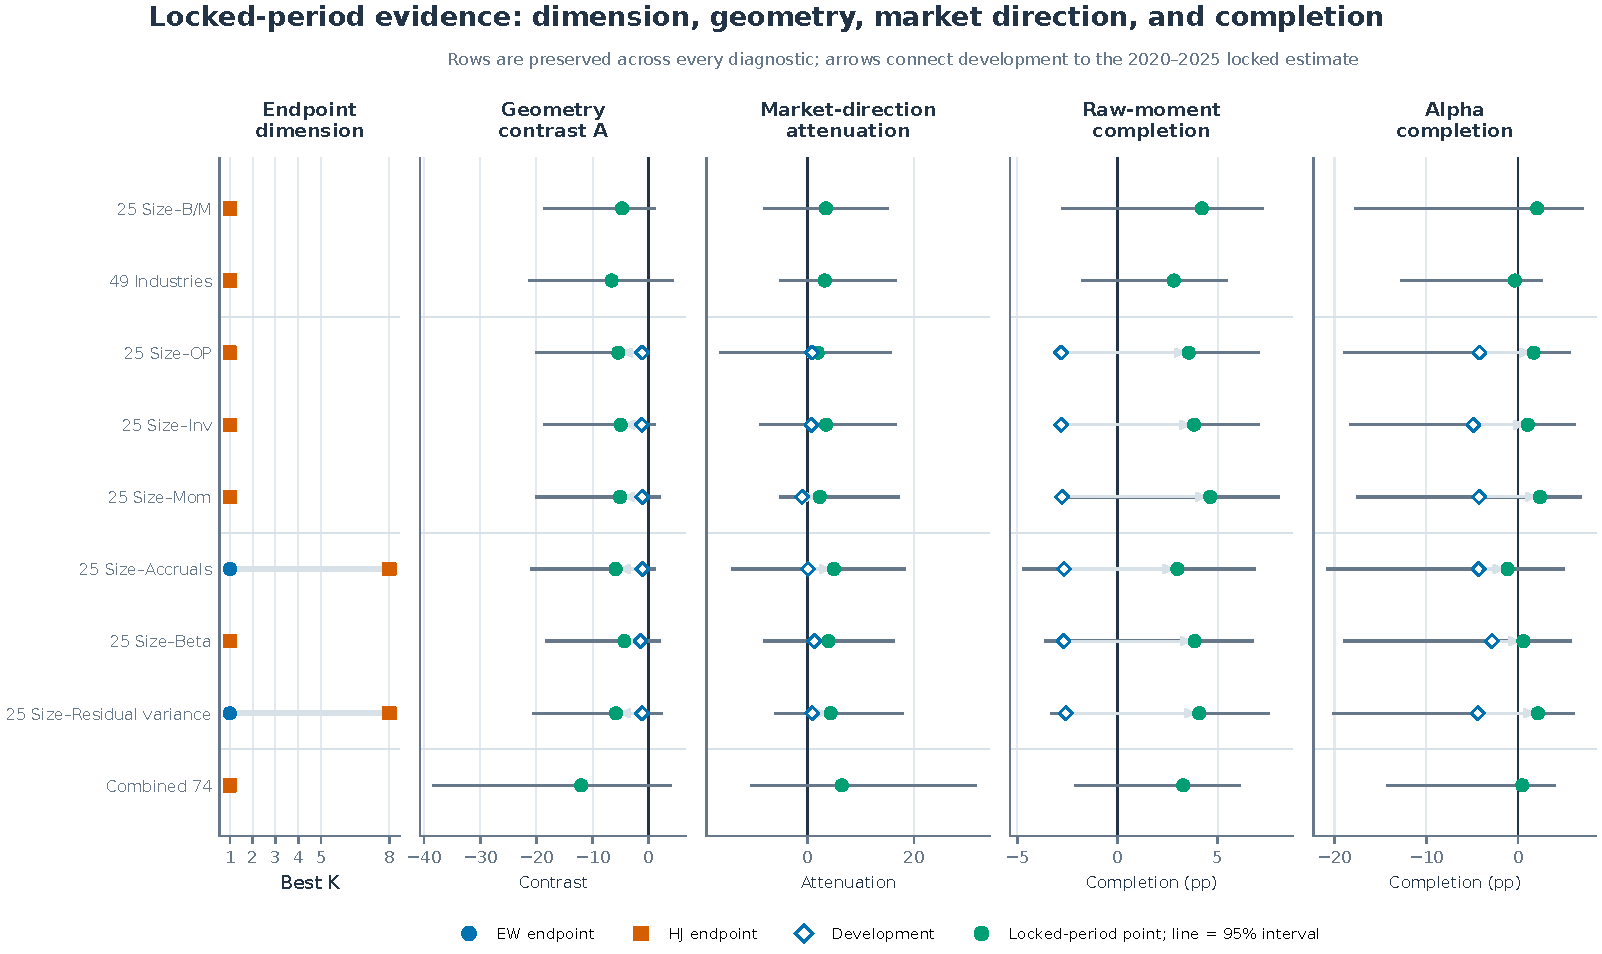
\includegraphics[width=0.99\textwidth]{figure_04_sealed_falsification.pdf}
\caption{Asset-aligned locked 2020--2025 evidence field. Each row preserves one test-asset family across endpoint dimension, raw geometry contrast $A$, market-direction attenuation, raw-moment completion, and alpha completion. Green points and horizontal lines report the locked estimate and its 95\% circular-block interval. For the six external families, hollow diamonds mark the development estimate and arrows point to the locked estimate. The first track compares equal-moment and HJ endpoint dimensions. The Core-86 models and rules were fixed before this later evaluation. Earlier legacy development includes January 2020; the period is not a wholly untouched research holdout. Plotting code was developed with OpenAI Codex assistance; the visualization is computed from archived data.}
\label{fig:sealed-dashboard}
\end{widefigure}

Table~\ref{tab:sealed-evidence} places each asset family's selected dimensions beside its pricing diagnostics and 95\% intervals. The locked point estimates have the anticipated market-attenuation sign but do not provide precise evidence of that effect or confirm the broader dimension pattern. The four frozen decisions follow directly from these rows. Geometry dependence fails because only two of six external families change endpoint dimension, below the four-family threshold, and Combined 74 does not change. The market-direction gate passes its point-estimate rule: attenuation is positive for Combined 74 and all six external families. Precision is limited because every corresponding block-bootstrap interval contains zero. Economic completion fails: no external family jointly improves raw moments and alpha. Dimension diversity fails because only $K=1$ and $K=8$ appear among external endpoint winners.



\begin{widetable}[!tbp]
\centering
\begin{minipage}{\textwidth}
\caption{Pricing dimensions and economic diagnostics in the locked 2020--2025 evaluation}
\label{tab:sealed-evidence}
\footnotesize
\setlength{\tabcolsep}{4pt}
\renewcommand{\arraystretch}{1.16}
\begin{tabular*}{\linewidth}{@{\extracolsep{\fill}}lccrrrr@{}}
\toprule
Test assets & \multicolumn{2}{c}{Best $K$} & Geometry & Market & \multicolumn{2}{c}{Completion (pp)} \\
\cmidrule(lr){2-3}\cmidrule(l){6-7}
 & EW & HJ & contrast $A$ & attenuation & Raw moments & Alpha \\
\midrule
\multicolumn{7}{@{}l}{\textit{Primary assets}} \\[2pt]
Size--B/M & 1 & 1 & -4.76 & 3.52 & 4.21 & 2.09 \\
 &  &  & [-18.76, 1.12] & [-8.15, 15.30] & [-2.80, 7.26] & [-17.85, 7.13] \\
Industries & 1 & 1 & -6.62 & 3.28 & 2.81 & -0.34 \\
 &  &  & [-21.32, 4.45] & [-5.11, 16.68] & [-1.82, 5.46] & [-12.85, 2.65] \\
Combined 74 & 1 & 1 & -12.04 & 6.48 & 3.28 & 0.48 \\
 &  &  & [-38.52, 4.11] & [-10.68, 31.74] & [-2.15, 6.16] & [-14.34, 4.10] \\
\addlinespace[4pt]
\multicolumn{7}{@{}l}{\textit{External assets}} \\[2pt]
Size--OP & 1 & 1 & -5.42 & 1.97 & 3.55 & 1.71 \\
 &  &  & [-20.16, -1.57] & [-16.47, 15.77] & [-3.06, 7.07] & [-19.07, 5.73] \\
Size--Inv & 1 & 1 & -5.00 & 3.54 & 3.82 & 1.07 \\
 &  &  & [-18.79, 1.11] & [-8.88, 16.66] & [-3.03, 7.06] & [-18.41, 6.27] \\
Size--Mom & 1 & 1 & -5.12 & 2.37 & 4.62 & 2.41 \\
 &  &  & [-20.16, 2.02] & [-5.11, 17.40] & [-2.94, 8.10] & [-17.58, 6.94] \\
Size--Accruals & 1 & 8 & -5.90 & 4.99 & 2.99 & -1.13 \\
 &  &  & [-20.99, 1.15] & [-14.19, 18.37] & [-4.73, 6.89] & [-20.89, 5.05] \\
Size--Beta & 1 & 1 & -4.36 & 3.97 & 3.85 & 0.59 \\
 &  &  & [-18.32, 2.14] & [-8.28, 16.33] & [-3.66, 6.78] & [-18.99, 5.86] \\
Size--Residual var. & 1 & 8 & -5.84 & 4.40 & 4.07 & 2.18 \\
 &  &  & [-20.71, 2.36] & [-6.18, 18.08] & [-3.35, 7.59] & [-20.26, 6.21] \\
\bottomrule
\end{tabular*}
\par\vspace{4pt}
{\footnotesize\raggedright\textit{Notes:} Brackets below each diagnostic are 95\% twelve-month circular-block bootstrap intervals (500 draws). Positive market attenuation means hedging reduces the absolute geometry contrast. Completion is the error of $K=1$ plus the market factor minus the error of $K=1$, multiplied by 100; negative values indicate improvement. EW and HJ denote the equal-moment and covariance-weighted endpoints. All rows use the frozen Core-86 models.\par}
\end{minipage}
\end{widetable}


The locked result narrows the interpretation of development evidence. Development evidence suggested broad geometry dependence. The locked period says that this pattern is not stable; one factor ranks first for most evaluated spans under the fixed models. This ranking alone does not identify a change in the economy's true risk count. The market-direction clue is more persistent in sign than the exact dimension ranking, but its uncertainty is too large for a strong structural claim. The last two tracks of Figure~\ref{fig:sealed-dashboard} make the development-to-locked completion reversal visible row by row across the six external families.

\subsection{Known-truth evidence on exact dimension recovery}

Feasible evaluation recovers the true dimension much less often than oracle evaluation. Table~\ref{tab:sim-mechanisms} separates the marginal selection frequencies (Panel A) from the eight prespecified mechanism contrasts (Panel B). All eight contrasts have the planned sign. Overall exact recovery is 64.2\% under oracle evaluation and 32.6\% under feasible evaluation. Increasing the sample from 72 to 600 months raises recovery from 38.1\% to 58.2\%, but the gain combines oracle and feasible designs and does not eliminate feasible over-selection. Strong risk prices raise recovery by 23.0 percentage points relative to weak prices. Full spanning raises it by 12.0 points relative to weak-tail spanning.

\begin{widetable}[!tbp]
\centering
\begin{minipage}{\textwidth}
\caption{Known-truth dimension selection: outcomes and prespecified mechanism contrasts}
\label{tab:sim-mechanisms}
\footnotesize
\setlength{\tabcolsep}{4pt}
\renewcommand{\arraystretch}{1.16}
\begin{tabular*}{\linewidth}{@{\extracolsep{\fill}}llrrrr@{}}
\toprule
\multicolumn{6}{@{}l}{\textit{A. Marginal selection outcomes}} \\[2pt]
Design axis & Level & Exact (\%) & Under (\%) & Over (\%) & Mean error \\
\midrule
Evaluation & Feasible & 32.6 & 33.9 & 33.5 & 1.693 \\
 & Oracle & 64.2 & 35.8 & 0.0 & 0.760 \\
\addlinespace[2pt]
Sample months & 72 & 38.1 & 46.2 & 15.7 & 1.526 \\
 & 240 & 48.9 & 34.4 & 16.8 & 1.197 \\
 & 600 & 58.2 & 23.9 & 17.8 & 0.956 \\
\addlinespace[2pt]
Risk prices & Strong & 59.9 & 22.1 & 17.9 & 0.900 \\
 & Weak & 36.9 & 47.5 & 15.6 & 1.552 \\
\addlinespace[2pt]
Asset spanning & Full & 54.4 & 28.6 & 16.9 & 1.105 \\
 & Weak tail & 42.4 & 41.0 & 16.6 & 1.347 \\
\addlinespace[2pt]
True dimension & 1 & 74.2 & 0.0 & 25.8 & 0.775 \\
 & 3 & 38.0 & 44.9 & 17.1 & 1.120 \\
 & 5 & 33.1 & 59.5 & 7.4 & 1.784 \\
\addlinespace[2pt]
Test assets & 25 & 46.8 & 36.7 & 16.5 & 1.257 \\
 & 74 & 50.0 & 33.0 & 17.0 & 1.195 \\
\addlinespace[2pt]
Factor correlation & 0.0 & 47.0 & 36.8 & 16.2 & 1.259 \\
 & 0.7 & 49.8 & 32.9 & 17.3 & 1.194 \\
\addlinespace[2pt]
Pricing geometry & Equal moments & 46.7 & 35.1 & 18.2 & 1.337 \\
 & HJ & 50.2 & 34.5 & 15.3 & 1.116 \\
\bottomrule
\end{tabular*}
\par\vspace{7pt}
\begin{tabular*}{\linewidth}{@{\extracolsep{\fill}}lrrr@{}}
\toprule
\multicolumn{4}{@{}l}{\textit{B. Prespecified mechanism contrasts}} \\[2pt]
Contrast and outcome & Cells & Effect (pp) & 95\% cell interval (pp) \\
\midrule
More time: exact recovery$^{a}$ & 24 & 26.5 & [17.8, 35.2] \\
Strong minus weak prices: exact recovery & 288 & 23.0 & [20.3, 25.7] \\
Weak minus strong prices: under-selection & 288 & 25.4 & [22.7, 28.1] \\
Full minus weak-tail span: exact recovery & 288 & 12.0 & [10.4, 13.6] \\
Weak-tail minus full span: asset-family divergence & 288 & 7.4 & [5.2, 9.6] \\
Equal--HJ disagreement: level$^{b}$ & 288 & 20.3 & [17.7, 22.9] \\
Complex minus baseline designs: disagreement$^{c}$ & 216 & 22.9 & [20.0, 25.9] \\
Oracle minus feasible evaluation: exact recovery & 288 & 31.6 & [29.0, 34.2] \\
\bottomrule
\end{tabular*}
\par\vspace{4pt}
{\footnotesize\raggedright\textit{Notes:} Panel A averages the remaining frozen design axes; its rows do not hold every other axis fixed. Exact, under-, and over-selection sum to 100\% before rounding; mean error is $|\widehat K-K_0|$. Oracle over-selection is zero by construction. Panel B uses percentage points (pp). Its archived intervals are the mean $\pm1.96$ standard errors across design-cell contrasts; they summarize cell heterogeneity, not uncertainty from independent Monte Carlo draws. $^{a}$600 minus 72 months, restricted to strong prices, full span, and $\rho=0$. $^{b}$An average level, not a difference. $^{c}$Correlation and/or weak-tail designs relative to full spanning with $\rho=0$. There are 500 Monte Carlo repetitions per base condition; six asset families share each repetition.\par}
\end{minipage}
\end{widetable}


Figure~\ref{fig:identification-dashboard} shows how recovery changes with sample length within each design. Panels A--B retain joint conditioning: rows separate risk-price strength and asset spanning, colors identify the true dimension, and line styles separate oracle from feasible evaluation. In the most favorable strong-price, full-span, zero-correlation design, oracle recovery at $T=600$ is 100\% for $K_0=1$, 99.8\% for $K_0=3$, and 99.2\% for $K_0=5$. These cells illustrate substantially better recovery when the evaluation mean is known. Feasible selection behaves differently. For $K_0=1$, recovery is approximately 46--51\% across 72, 240, and 600 months under the two geometries. Its over-selection probability does not vanish.

\begin{widefigure}[!tbp]
\centering
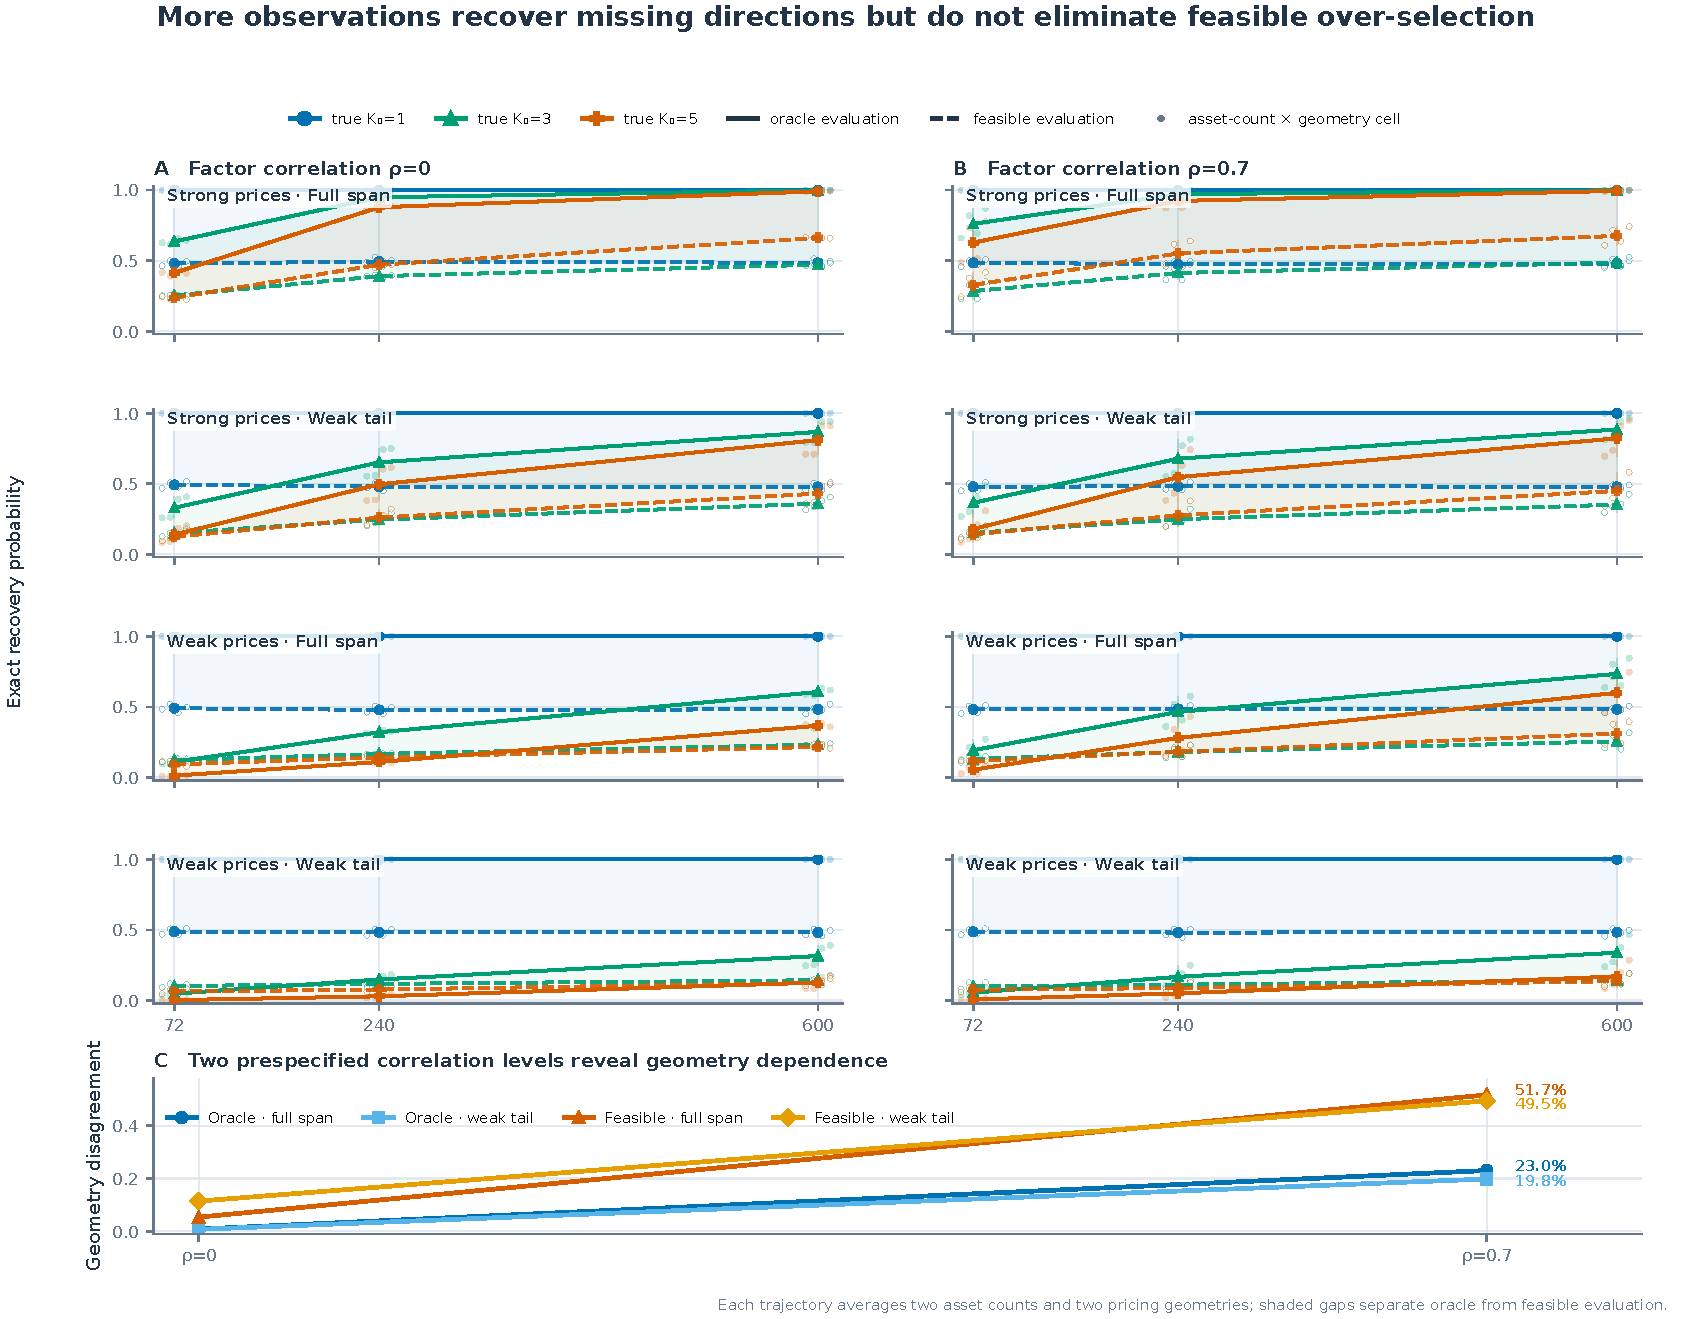
\includegraphics[width=0.99\textwidth]{figure_05_identification_mechanisms.pdf}
\caption{Known-truth identification trajectories over the complete frozen condition grid. Panels A and B plot exact recovery at the three prespecified sample lengths, 72, 240, and 600 months, under factor correlations zero and 0.7. Rows distinguish risk-price strength and asset spanning; colors identify $K_0$; solid and dashed lines separate oracle and feasible evaluation. Small points expose the four asset-count--pricing-geometry cells behind each mean marker; their vertical range is also shown. Each mean is therefore based on 12,000 selection outcomes. Shaded gaps show the loss from feasible evaluation. Panel C is a two-level slope graph, rather than an interpolated correlation curve, and reports equal-versus-HJ dimension disagreement at the two prespecified correlation values. Plotting code was developed with OpenAI Codex assistance; the visualization is computed from archived data.}
\label{fig:identification-dashboard}
\end{widefigure}

The result illustrates Proposition~\ref{prop:inconsistency}. Models above $K_0$ add directions with zero population price. Their empirical losses fluctuate around the same population value, so the strict minimum rewards whichever redundant direction happens to reduce sample loss. More data shrink all differences, but they do not force the sign of a centered, second-order difference to favor the minimal model. In the aggregate feasible design, the over-selection rate is 33.5\%; it rises from 31.3\% at 72 months to 35.7\% at 600 months rather than disappearing.

\subsection{Asset spanning and geometry disagreement}

Weak-tail spanning reduces the loadings on the final true directions to 0.15 of their baseline magnitude. Exact recovery falls by 12.0 percentage points, and the probability that six asset families select different dimensions rises by 7.4 points. Under oracle evaluation, multiple dimensions appear across the six families in 27.8\% of strong/full conditions, 55.1\% of strong/weak-tail conditions, and about 63--65\% of weak-price conditions. Under feasible evaluation, cross-family diversity appears in 98--99\% of conditions. A common economic dimension can therefore generate heterogeneous empirical dimensions when assets reveal its weaker directions unevenly.

Equal and HJ geometries disagree on the selected dimension in 20.3\% of all simulation cases. With independent factor directions and full spanning, disagreement is only 0.8\% under oracle evaluation and 5.3\% under feasible evaluation. Raising factor correlation to 0.7 increases those rates to 23.0\% and 51.7\%. Panel C of Figure~\ref{fig:identification-dashboard} displays this amplification.

The simulation does not identify which mechanism causes each empirical result. It establishes that the specified combinations of weak prices, weak spanning, correlated risks, weighting, and evaluation noise can generate unstable selection. The design contrasts do not imply that each mechanism alone explains the empirical results. It would be invalid to invert the simulation and declare the true empirical dimension or the causal share of each mechanism.

\subsection{Descriptive loss-tolerance sets}

A candidate minimum can be accompanied by a transparent loss-tolerance set,
\begin{equation}
 \widehat{\mathcal A}_{\delta}^{\mathrm{desc}}=
 \{K:\widehat\Loss(K)-\min_j\widehat\Loss(j)\leq\delta\}.
\end{equation}
Here $\delta$ is a stated descriptive tolerance, not a critical value. This set
reports proximity to the observed minimum. It is neither a confidence set for
the population minimizer nor evidence of statistical or economic equivalence.
The conditional-autoencoder archive uses a fixed tolerance of 1\% of the
FF5-plus-momentum development distance and retains the full candidate losses.
That convention has no claim to being a universally appropriate economic
threshold. A formal equivalence claim would require a justified margin and
valid uncertainty assessment for the corresponding estimand. The failed
calibration in \ref{app:inference-calibration} prevents the new
simultaneous intervals from supplying that assessment here.

\section{What does the network geometry establish?}
\label{sec:geometry}

\subsection{Absolute rank, layer width, and an architecture control}

Absolute participation rank falls with depth, but hidden width also contracts from 128 to 64 to 32. The archived raw-centered medians are 20.251, 14.669, and 9.048 (Table~\ref{tab:geometry}). Dividing by width gives 15.8\%, 22.9\%, and 28.3\%, respectively. Thus the absolute decline does not show increasing concentration relative to the available coordinates. Feature z-scoring and row-$L_2$ normalization retain the absolute ordering, but cannot remove the architecture comparison by themselves.

A bounded supplementary control compares the 30 frozen trained networks with five untrained networks on exactly the same 384 securities in each of the 120 development months. Architecture, activation functions, input preprocessing, and seed identifiers match; the untrained hidden weights for a seed are shared across all six output dimensions rather than counted as six independent random networks. These are fresh draws under the recorded control runtime, not a recovery of the exact historical initialization tensors. The design was fixed before its execution, after the earlier manuscript and diagnostics were available.

The control separates two observations (Figure~\ref{fig:geometry-dashboard}). Random networks already have falling mean absolute ranks: 20.435, 15.253, and 10.399. Trained means are 20.318, 14.114, and 8.691. Training is associated with additional concentration, especially in the last two layers. The primary final-layer mean rank/width difference is $-5.340$ percentage points, with a paired 95\% interval of $[-7.737,-3.359]$. It uses 1,000 common twelve-month circular-block draws with paired seed resampling, retaining every $K$ within its seed. The interval is conditional on the archived networks and sample; five initializations limit generalization. The sign supports training-associated concentration beyond this random-network benchmark, not identification of a pricing dimension.

\begin{widetable}[!tbp]
\centering
\begin{minipage}{\textwidth}
\caption{Trained and random-network concentration on matched inputs}
\label{tab:architecture-control}
\footnotesize
\setlength{\tabcolsep}{4pt}
\renewcommand{\arraystretch}{1.16}
\begin{tabular*}{\linewidth}{@{\extracolsep{\fill}}crrrrr@{}}
\toprule
Layer & Width & Trained PR & Random PR & Gap / width (pp) & 95\% interval \\
\midrule
\multicolumn{6}{@{}l}{\textit{A. Raw centered}} \\[2pt]
H1 & 128 & 20.318 & 20.435 & -0.092 & [-0.214, 0.063] \\
H2 & 64 & 14.114 & 15.253 & -1.780 & [-2.596, -1.059] \\
H3 & 32 & 8.691 & 10.399 & -5.340 & [-7.737, -3.359] \\
\addlinespace[4pt]
\multicolumn{6}{@{}l}{\textit{B. Feature z-score}} \\[2pt]
H1 & 128 & 23.057 & 23.138 & -0.064 & [-0.175, 0.092] \\
H2 & 64 & 16.204 & 17.219 & -1.587 & [-2.229, -1.014] \\
H3 & 32 & 10.241 & 11.755 & -4.729 & [-6.667, -3.041] \\
\addlinespace[4pt]
\multicolumn{6}{@{}l}{\textit{C. Row-$L_2$}} \\[2pt]
H1 & 128 & 21.131 & 21.270 & -0.108 & [-0.217, 0.028] \\
H2 & 64 & 14.926 & 15.950 & -1.600 & [-2.412, -0.865] \\
H3 & 32 & 8.793 & 10.448 & -5.170 & [-7.412, -3.320] \\
\bottomrule
\end{tabular*}
\par\vspace{4pt}
{\footnotesize\raggedright\textit{Notes:} PR denotes participation rank. Entries are means, unlike the archived medians in Table~\ref{tab:geometry}. Width-normalized gaps are trained minus random. The primary endpoint is raw-centered H3; all other rows are descriptive. The 1,000 draws resample common twelve-month circular blocks and five paired seed clusters. Random hidden weights are shared across all six $K$ values. Intervals are pointwise and conditional on the archived sample and trained weights. This control was designed after the earlier study; it does not retune the economic-function probe.\par}
\end{minipage}
\end{widetable}


\begin{widetable}[!tbp]
\centering
\begin{minipage}{\textwidth}
\caption{Layerwise representation geometry under three normalization rules}
\label{tab:geometry}
\footnotesize
\setlength{\tabcolsep}{4pt}
\renewcommand{\arraystretch}{1.16}
\begin{tabular*}{\linewidth}{@{\extracolsep{\fill}}lrrrrrrr@{}}
\toprule
Layer & Participation & Entropy & PCA95 & TWO-NN & LB ($k=20$) & Tangent angle & Drift \\
 & rank & rank & rank & dimension & dimension & (radians) & (rank 5) \\
\midrule
\multicolumn{8}{@{}l}{\textit{A. Raw centering}} \\[2pt]
Hidden 1 & 20.251 & 35.855 & 50 & 15.477 & 13.835 & 1.493 & 0.987 \\
Hidden 2 & 14.669 & 23.760 & 32 & 14.072 & 12.054 & 1.474 & 0.862 \\
Hidden 3 & 9.048 & 13.839 & 18 & 11.814 & 9.757 & 1.437 & 0.670 \\
\addlinespace[5pt]
\multicolumn{8}{@{}l}{\textit{B. Feature z-score}} \\[2pt]
Hidden 1 & 22.989 & 38.444 & 51 & 15.750 & 14.186 & 1.494 & 0.942 \\
Hidden 2 & 16.538 & 25.430 & 32 & 14.237 & 12.399 & 1.477 & 0.890 \\
Hidden 3 & 10.476 & 15.097 & 18 & 11.990 & 10.058 & 1.429 & 0.661 \\
\addlinespace[5pt]
\multicolumn{8}{@{}l}{\textit{C. Row-$L_2$ normalization}} \\[2pt]
Hidden 1 & 21.168 & 36.728 & 50 & -- & -- & -- & 0.948 \\
Hidden 2 & 15.479 & 24.609 & 32 & -- & -- & -- & 0.856 \\
Hidden 3 & 9.105 & 13.903 & 18 & -- & -- & -- & 0.661 \\
\bottomrule
\end{tabular*}
\par\vspace{4pt}
{\footnotesize\raggedright\textit{Notes:} Entries are archived medians for 30 frozen networks and 120 development months. Spectral summaries use 3,600 observations per group; drift uses 3,570 adjacent-month pairs. Neighbor dimensions and tangent angles use only 300 observations per raw/z-score group (ten sampled months). LB is the Levina--Bickel estimator. Dashes denote diagnostics not computed under row normalization, not zero values. The numerical-collapse rate is zero; it is not a classification neural-collapse test. The two adjacent-layer CKA medians are 0.875 and 0.848. These are descriptive, finite-scale diagnostics; the separate economic-function test is reported in Figure~\ref{fig:evidence-ladder} and Section~\ref{sec:function-gate}.\par}
\end{minipage}
\end{widetable}


Independent synthetic calibration precedes the empirical estimates. The first calibration failed two of six gates because a fixed tangent-space rank could not distinguish curved from flat manifolds and the scale-artifact design did not match the z-score estimand. Those failures were retained. A corrected, frozen calibration chose local rank adaptively and aligned the scale design with the estimand; it passed plane dimensions 3 and 8, curvature, collapse, scale-artifact, and full-rank anisotropy gates. This supports use of the estimators as directional diagnostics, not as an oracle for unique intrinsic dimension.

The collapse rate is zero. The final layer's leading-eigenvalue share is 0.232 and its PCA90 and PCA95 dimensions are 14 and 18. Hence the pattern is anisotropic concentration rather than a representation converging to a constant or a one-dimensional line. Z-scoring increases final-layer participation rank by 1.427, or 15.8\%, which confirms some scale influence but remains far below the frozen 50\% artifact threshold.

\subsection{Concentration is not evidence of a smooth pricing manifold}

The term ``manifold'' suggests more than a low effective rank. It suggests that observations lie near a smooth lower-dimensional object whose local tangent spaces vary coherently. The finite-scale tangent-angle diagnostic is insufficient to establish that interpretation. Its median declines from 1.493 to 1.437 radians rather than increasing with depth. Values near a right angle indicate that local and larger-scale tangent estimates are not tightly aligned. The representation is concentrated, but the evidence does not establish a unique smooth manifold.

Adjacent-layer CKA medians are 0.875 for hidden 1 versus hidden 2 and 0.848 for hidden 2 versus hidden 3. Layers retain much of the same cross-sectional structure while reorganizing it. Rank-five monthly Grassmann drift falls from 0.987 to 0.862 and 0.670 across layers. Deeper principal subspaces are more stable over adjacent months even though they are not fixed.

High-volatility months have a final-layer raw participation rank only 0.165 above other months. The small association does not identify a volatility-driven state transition. It also illustrates why a geometrically stable subspace and a stable pricing function are different claims: the subspace can move less while the output weights or realized price of risk change materially.

\subsection{The prespecified economic-function gate fails}
\label{sec:function-gate}

The separate economic-function criterion is not met. The architecture control does not change this previously specified test or its endpoint. Figure~\ref{fig:evidence-ladder} displays the model-level prediction errors. The primary probe predicts each model's development-period HJ loss from final-layer geometry after controlling for nominal factor count. Validation leaves out one seed at a time so that a seed-specific geometry--performance relation cannot be evaluated on the same seed used to fit it. Adding geometry reduces RMSE from 0.106 to 0.102, an improvement of 3.915\%. This is below the prespecified 5\% threshold, and the within-factor-count permutation $p$-value is 0.149. The within-factor-count Pearson correlation is $-0.296$.

The secondary factor-Sharpe endpoint has permutation $p=0.041$ but improves RMSE by only 1.211\%. It cannot replace the failed HJ endpoint. Searching another layer, normalization, state split, or economic outcome after seeing the result would convert a prespecified test into an unbounded geometry search. The analysis therefore stops at the planned gate.

\begin{widefigure}[!tbp]
\centering
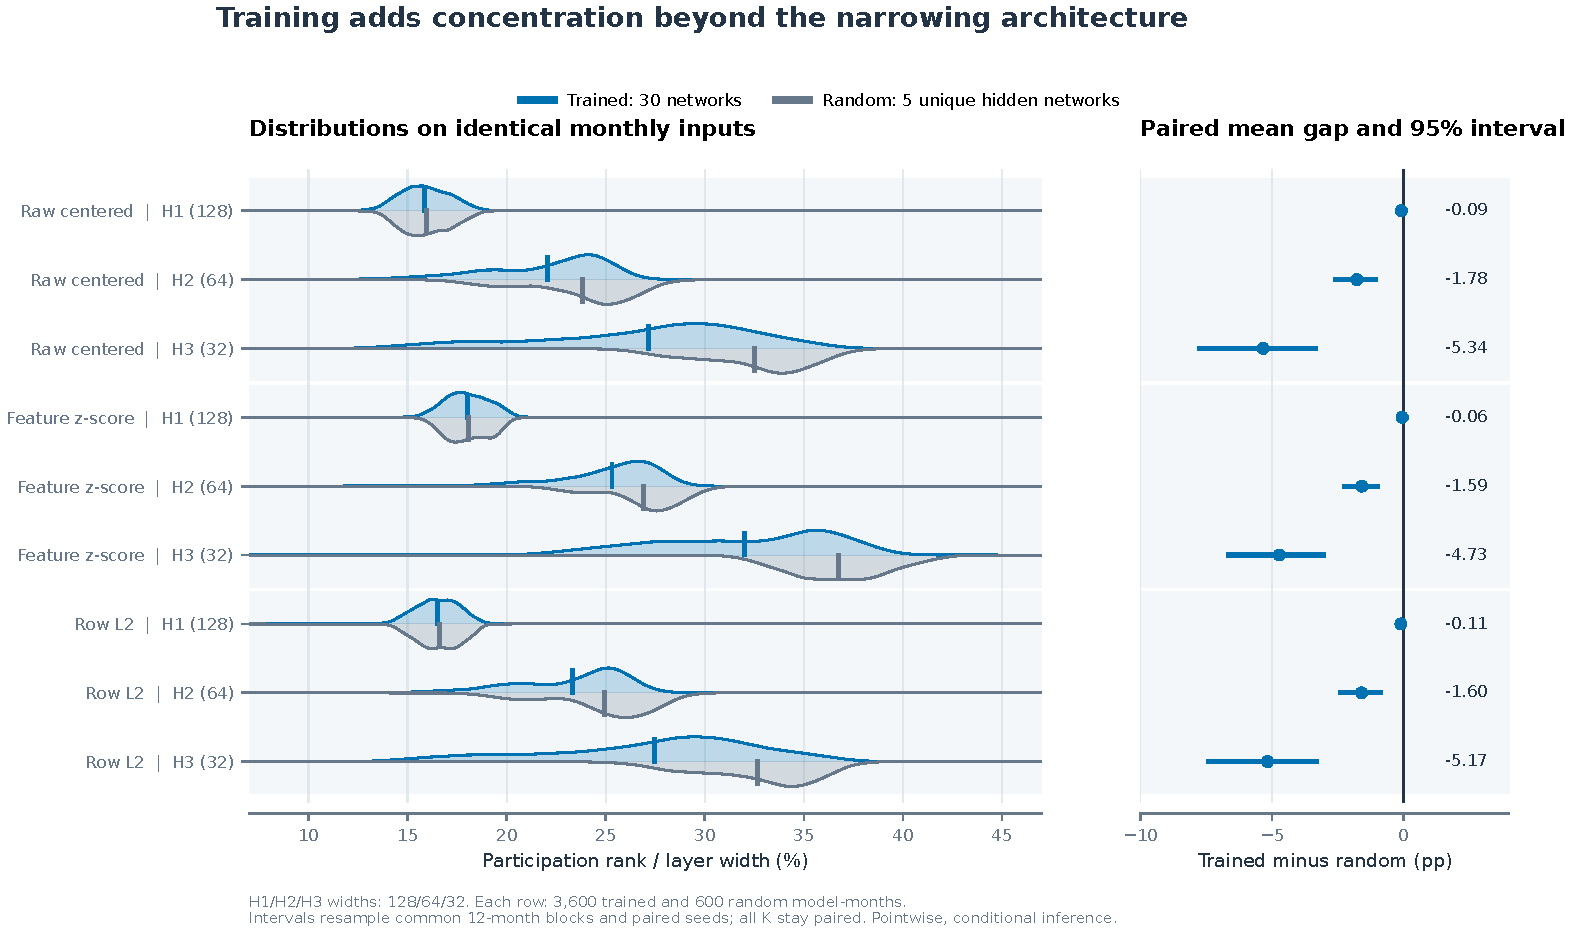
\includegraphics[width=0.98\textwidth]{figure_07_geometry_function.pdf}
\caption{Architecture-matched representation control. Each row compares participation rank divided by layer width for the original diagnostic networks and matched random networks on the same monthly inputs. The later conditional-autoencoder models are not included. There are 3,600 trained and 600 unique random observations per row; random hidden weights are shared across $K$. Markers show means. The aligned right-hand intervals report trained-minus-random mean differences in percentage points under paired twelve-month block and seed resampling. These are pointwise descriptive intervals. Absolute rank falls even in random networks; the training-associated gap is a separate comparison from the failed economic-function probe in Figure~\ref{fig:evidence-ladder}. Plotting code was developed with OpenAI Codex assistance; the visualization is computed from archived data.}
\label{fig:geometry-dashboard}
\end{widefigure}

The result clarifies what high-dimensional networks may be doing. They map 86 characteristics and 86 missingness indicators into anisotropic hidden coordinates. Absolute rank declines as layers narrow, and training adds concentration relative to matched random networks. Rank-five subspaces also move less between adjacent months in deeper layers. But concentration does not reveal the number of priced shocks. It may reflect denoising, redundancy removal, saturation, common firm-characteristic structure, or an architecture-induced spectral bias. For the proposed incremental pricing interpretation, the geometry must predict pricing moments, SDF performance, or exposure spans beyond what nominal factor count already explains. The prespecified probe does not provide that incremental evidence here.

\subsection{Connecting geometric and economic compression}

The empirical pieces are consistent without being identical. The hidden representation concentrates to an effective rank near nine, while endpoint pricing choices range among one, two, four, five, and eight depending on data and loss. There is no contradiction: effective rank counts active variation in hidden activations, whereas pricing dimension counts directions needed to reduce a particular set of Euler errors. Some active hidden directions can support nonlinear sorting without carrying distinct risk prices. Some weak priced directions can have little activation variance and still matter under an HJ geometry or for a targeted asset family.

The economic direction of compression provides the bridge. Development decompositions show that a dominant common payoff direction explains part of the geometry contrast. The hidden-state evidence shows a broad anisotropic representation rather than a literal one-factor code. One interpretation is that a few common directions contain much of the variation, while additional directions may refine relative pricing. These diagnostics do not identify that hierarchy within individual hidden units. Which refinement counts as necessary depends on asset spanning, the metric, measurement, and the historical risk-price configuration.

These distinctions motivate reporting a spectrum, descriptive loss gaps or a stated tolerance set, and economic labels only for directions supported by the design. In the original diagnostics, the common market-direction point estimates retain a sign more consistently than the exact validation minimum; their wide intervals limit a stronger comparison. That is the sense in which compression can be economically interpretable without being a stable law of exact dimension.

\section{Discussion and conclusion}

\subsection{What the controls change}

The experiments distinguish concentration in activations, selection within a candidate grid, and an economic factor count. In the original diagnostic family, rankings change across assets, weighting, archived pipelines, seeds, and periods. The matched controls narrow the explanation: absolute rank also falls in random networks as layers narrow, training adds concentration beyond that benchmark, and removing six features on a common panel does not reproduce the archived pipeline reversal. The original contrast cannot be assigned to feature deletion alone.

The conditional-autoencoder extension changes the scope of the selection result. Its point-estimate diagnostics are favorable relative to the chosen reference, and selection is concentrated at $K=8$ in the fixed grid. The study therefore contains both sensitive and comparatively concentrated selections. It does not establish universal dimension instability among successful pricing models. Because eight is the largest candidate, the result also does not identify a global optimal width. A finite-grid preference and the number of priced structural shocks remain different objects even when that preference is stable. The complete archived secondary surface strengthens this boundary: eight factors minimize all fifteen autoencoder asset--weight tasks, whereas the matched linear-loading minima move across four, five and eight. Endpoint-transfer costs in the latter range from 2.09\% to 9.34\%. This architecture dependence prevents a universal instability claim.

Inference further limits the interpretation. All 15 exploratory pairwise intervals include zero, but the primary known-truth calibration exhibits undercoverage. We retain that result and do not use non-rejection as evidence of equivalence or structural nonidentification. The failure is specific to the tested procedure and moment designs; it does not estimate empirical error probabilities or invalidate every other procedure in the study. Nor is it an economic explanation for why a dimension changes. Its role is to delimit the inferential claims available from the extension.

\subsection{Economic interpretation and reporting}

The original market-direction diagnostics suggest a distinction between dominant common payoff variation and relative-pricing errors. Removing a validation-estimated market component attenuates the geometry contrast in later-period point estimates, while adding the market factor does not jointly improve raw moments and alphas. Wide attenuation intervals and pipeline sensitivity prevent precise causal attribution of compression losses to market risk. We do not estimate the separate contributions of state complexity, risk exposures, or risk prices.

For empirical reporting, a selected width should be accompanied by the candidate loss profile, its payoff span and weighting, and algorithmic dispersion. A stated tolerance can summarize small observed gaps, but cannot establish equivalence without a justified margin and valid inference. Losses computed using evaluation-estimated weights in the original diagnostic exercise and validation-fixed weights in the conditional-autoencoder extension should not be combined into a model league table. Each comparison is interpreted within its own fixed evaluation protocol.

\subsection{Limitations}

The original pricing family failed earlier benchmark-advancement criteria. The later conditional-autoencoder control improves benchmark relevance by the prespecified point-estimate diagnostic, but does not establish state-of-the-art performance, superiority to its matched linear-loading arm, or a representative result for all neural pricing architectures. All results concern U.S. equities, conventional numerical characteristics, and the specified asset spans.

Chronology restricts confirmation claims. Legacy development included January 2020 before the 2020--2025 exercise was locked. The feature, architecture, conditional-autoencoder, and inference controls were designed after inspection of earlier findings. Their frozen run protocols limit further search but do not make the historical data new. The conditional-autoencoder extension does not access 2020--2025. None of these controls is described as an independent prospective replication.

The characteristic bridge retains benchmark values where available and reconstructed values otherwise. It is not an independent point-in-time vintage archive. Accounting revisions, coverage, and timing may affect rankings. The matched feature control preserves 184 input positions, rather than recreating the original 172-input architecture; its conclusions are conditional on that parameterization. Licensed security-level data cannot be included in the public package, so aggregate exhibit replay and licensed-data reconstruction are separate reproducibility tasks.

Geometry is measured at a finite cross-sectional sample and neighborhood scale. The tangent-angle diagnostic does not identify a unique smooth pricing manifold. Random-network comparisons use five fresh initialization draws rather than recovered original initial tensors; the functional probe contains 30 models and five seed folds. Its failed threshold does not prove that geometry contains no economic information. The known-loading simulation and penalty calculation concern a finite nested Gaussian family, not separately fitted neural networks. The new inference calibration conditions on fixed models and weights and does not reproduce uncertainty from the full training pipeline.

\subsection{Conclusion}
Dimension selection should be reported together with its target loss and the cost of alternative candidates. In the archived diagnostic networks, carrying the preferred count between weighting endpoints can have asymmetric norm costs. A same-panel control excludes six-feature deletion as a sufficient explanation of the older pipeline reversal. The conditional-autoencoder results show concentrated selection and larger descriptive losses from stronger compression, while the linear-loading comparison shows smaller marginal costs near the upper grid endpoint. These results support task-specific reporting; they do not establish a true economic risk count or a universally unstable neural representation. Simulated mechanisms and imprecise market-direction evidence remain distinct from empirical causal attribution. The separate interval-calibration failure limits formal inference, and future work on valid inference is not presented as completed here.


\section*{Funding}
This research received no specific grant from any funding agency in the public, commercial, or not-for-profit sectors.

\section*{Declaration of competing interest}
The authors declare that they have no known competing financial interests or personal relationships that could have appeared to influence the work reported in this paper.

\section*{CRediT authorship contribution statement}
\textbf{Jinpeng Wang:} Conceptualization, Methodology, Software, Data curation, Formal analysis, Visualization, Writing -- original draft, Writing -- review \& editing.
\textbf{Yan Jiang:} Supervision, Validation, Writing -- original draft, Writing -- review \& editing.


\section*{Data availability}
The replication package provides construction and analysis code, frozen configurations, synthetic results, aggregate figure and table data, and checksums. The section-ordered package includes the conditional-autoencoder control (P1-G4-V003) and its inference calibration (P1-G4-V004), including unsuccessful calibration results. CRSP, Compustat, CCM, third-party security-level characteristic records, model checkpoints, stock-level predictions, and derived security-level panels are excluded. Reconstruction requires independently licensed inputs. Public source downloads are linked rather than relicensed. Aggregate exhibit replay is separate from retraining with licensed data, and no cross-platform bitwise retraining guarantee is made.

Version 1.3.0 of the replication package is available at \href{https://doi.org/10.5281/zenodo.24398249}{10.5281/zenodo.24398249}. It includes this manuscript, the separate audit supplement, all 900 frozen aggregate surface rows, 180 candidate means, 30 task summaries, 12 endpoint transfers, and the public arithmetic-replay script. The GitHub project is \href{https://github.com/extradimen/asset-pricing-dimension-replication}{https://github.com/extradimen/asset-pricing-dimension-replication}; the version-specific Zenodo archive identifies the exact files supporting this revision. Version 1.2.1 and its original identifiers are preserved within the package and remain separately available at \href{https://doi.org/10.5281/zenodo.23177771}{10.5281/zenodo.23177771}.

\section*{Declaration of generative AI and AI-assisted technologies in the manuscript preparation process}
During the preparation of this work, the authors used OpenAI Codex to assist with literature organization, code development and auditing, artifact indexing, statistical-figure production, and language drafting. The authors reviewed and edited all generated material, verified cited sources and numerical claims against frozen project evidence, and take full responsibility for the content of the article.

\begingroup
\small
\raggedright
\setlength{\bibsep}{3pt}
\urlstyle{same}
\bibliographystyle{rQUF}
\bibliography{references_qf}
\endgroup
\appendix
\setcounter{table}{0}
\renewcommand{\theHtable}{A.\arabic{table}}
% IREF working appendix fragment; all numbers copied from frozen V004 outputs.
% Requires booktabs. No replacement for the archived V003/V004 numerical files.
\section{Calibration of the exploratory dimension-comparison intervals}
\label{app:inference-calibration}

Experiment P1-G4-V004 evaluates the previously fixed simultaneous-interval
procedure without fitting additional networks or examining additional empirical
periods. Six candidate labels and five model variants are represented by pricing
moment vectors with known population means. After a fixed whitening transform,
their population distance is $d_{ks}=\sqrt{12}\|\mu_{ks}\|_2$. Deterministic
rotations give the five variants the same population distance within each
candidate. Stationary Gaussian AR(1) innovations combine common, candidate, and
variant components with variance shares 0.5, 0.3, and 0.2. Total innovation energy
is held constant across moment ranks. This is a moment-level calibration,
conditional on fixed models and weights, rather than a structural return/SDF
model or an estimate of power for the empirical panel.

For each simulated sample, we reproduce the original procedure: common
12-month circular time blocks, five jointly resampled variant indices, the
average of variant-specific sample distances, and all 15 pairwise differences.
For difference $j$, let $\widehat\Delta_j$ be its point estimate,
$\widehat\Delta_j^{*(b)}$ its bootstrap value, and $s_j^*$ the bootstrap standard
deviation. The common critical value is the 0.95 bootstrap quantile of
$\max_j |(\widehat\Delta_j^{*(b)}-\widehat\Delta_j)/s_j^*|$; the interval is
$\widehat\Delta_j\pm c_{.95}s_j^*$. This is a single-step maximum standardized
bootstrap-deviation construction. It does not re-estimate the standardizer
inside each draw and does not implement a stepdown procedure.

The frozen design contains 30 scenarios, each with 400 independently seeded
outer replications and 1,999 inner draws. The primary scenarios use 74 moment
coordinates, 120 months, baseline distance five, AR coefficients zero or 0.5,
and population gaps of zero, 0.5, one, or two between the first five candidates
and the sixth. Prespecified sensitivities extend the sample to 240 or 600 months,
reduce the moment rank to four, or set all distances to zero. Candidate labels
do not represent a known structural factor count. The design contains no
post-calibration adjustment to the block length, candidate grid, or interval
construction.

\begin{widetable}[!tbp]
\centering
\caption{Equal-distance calibration: simultaneous coverage and familywise rejection}
\label{tab:inference-calibration}
\small
\begin{tabular}{rrrrrr}
\toprule
Months & Rank & Distance & AR coefficient & Coverage (\%) & FWER (\%) \\
\midrule
120 & 74 & 5 & 0.0 & 83.50 & 16.50 \\
120 & 74 & 5 & 0.5 & 87.00 & 13.00 \\
240 & 74 & 5 & 0.0 & 91.50 & 8.50 \\
240 & 74 & 5 & 0.5 & 91.75 & 8.25 \\
600 & 74 & 5 & 0.0 & 93.25 & 6.75 \\
600 & 74 & 5 & 0.5 & 93.00 & 7.00 \\
120 & 4 & 5 & 0.0 & 86.25 & 13.75 \\
120 & 4 & 5 & 0.5 & 90.50 & 9.50 \\
120 & 74 & 0 & 0.0 & 98.75 & 1.25 \\
120 & 74 & 0 & 0.5 & 98.50 & 1.50 \\
\bottomrule
\end{tabular}
\par\smallskip
\begin{minipage}{0.96\linewidth}\footnotesize
Each row contains 400 outer replications. Coverage requires all 15 intervals
to include their population differences. FWER is the probability of excluding
zero in at least one comparison; since all differences in these rows equal
zero, it equals one minus simultaneous coverage. Nominal values are 95\%
coverage and 5\% FWER. Wilson Monte Carlo 95\% intervals for coverage in the
first two rows are [79.55,86.82]\% and [83.35,89.95]\%; the corresponding FWER
intervals are [13.18,20.45]\% and [10.05,16.65]\%. These probabilities describe
the specified simulations, not empirical error probabilities for U.S. equities.
All 30 scenarios, including unequal-distance detection results, are retained
in the experiment archive.
\end{minipage}
\end{widetable}

The primary short-sample equal-distance scenarios exhibit undercoverage and
excess familywise rejection. Longer samples improve coverage in those scenarios
but do not establish exact calibration. The two zero-distance stress scenarios
are conservative, so the primary failures cannot be attributed simply to the
norm's nondifferentiability at zero. The experiment does not isolate the
contributions of block length, nonlinear transformation, dependence, and
variant resampling. In particular, the fixed rotated variants do not reproduce
the distribution of repeatedly trained networks. These limits restrict the
interpretation of the calibration without removing its adverse result.

This exercise does not calibrate the separate predictive-$R^2$ intervals,
the pointwise difference from FF5 plus momentum, or the earlier paper's other
procedures. Nor does failure of this particular construction establish a new
economic mechanism. Its consequence is narrower: the exploratory simultaneous
intervals are not used to support equivalence, a confidence set for a unique
dimension, or structural nonidentification. Point estimates and all original
outputs remain reported without retuning the empirical models.



\end{document}
